\part{第2講：インフレーション中の{\sl 量子}揺らぎ}


\vspace{0.5cm}
 \hrule \vspace{0.3cm}
\begin{quote}
{\bf 要旨}

\noindent
本講では，インフレーション中の量子揺らぎが生成する原始揺らぎのスペクトルについて，よく知られた計算を示す．
計算の細部をすべて示し，「ごまかし」や近似をできるだけ避ける．
宇宙論的摂動論の基礎を簡単に復習した後，まず，インフレーションが微視的な量子揺らぎを宇宙の構造形成の巨視的な種へ変換する基本機構を定性的にまとめる．
次に，曲がった時空における場の量子論への教育的な導入として，単純調和振動子の量子化を復習する．真空が最低エネルギー状態であることを要求すると，真空状態が一意に選ばれる点を強調する．
続いて，インフレーションについて対応する計算を行う．
スカラー揺らぎとテンソル揺らぎの両方のパワースペクトルを計算し，そのスケール依存性を論じる．

\end{quote}
\vspace{0.1cm}  \hrule
 \vspace{1.5cm}



前講では，ポテンシャルを速度$\dot \phi$で転がり落ちるスカラー場の古典的（$\hbar =0$）な力学を調べた（図\ref{fig:small2}参照）．本講では，古典的な背景の時間発展$\bar \phi(t)$の周りの量子（$\hbar \ne 0$）揺らぎの効果を調べる．この揺らぎは，インフレーションの終了時刻に局所的な遅延を生む．すなわち，宇宙の異なる領域では，インフレーションがわずかに異なる時刻に終わる．例えば，図\ref{fig:small2}のポテンシャルでは，凍結した負の揺らぎ$\delta \phi$を獲得した領域は，正の$\delta \phi$をもつ領域より長くポテンシャルが支配的な状態にとどまる．
したがって，宇宙の異なる領域はわずかに異なる時間発展をたどる．これが相対的な密度揺らぎ$\delta \rho(t, {\bf x})$を生む．
%These fluctuations persist after inflation and provide the initial conditions for the formation of large-scale structures.

\begin{figure}[htbp]
    \centering
        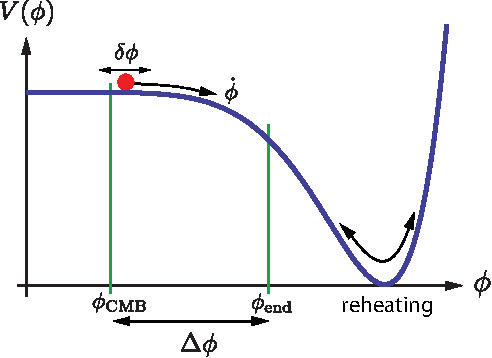
\includegraphics[width=0.4\textwidth]{SmallField}
   \caption{\small 古典的な背景の時間発展$\bar \phi(t)$の周りの量子揺らぎ$\delta \phi(t, {\bf x})$．}
    \label{fig:small2}
\end{figure}

本講では，大規模構造の量子的起源についてのこの基本描像を支える技術的な詳細を論じる．


\begin{figure}[h!]
    \centering
        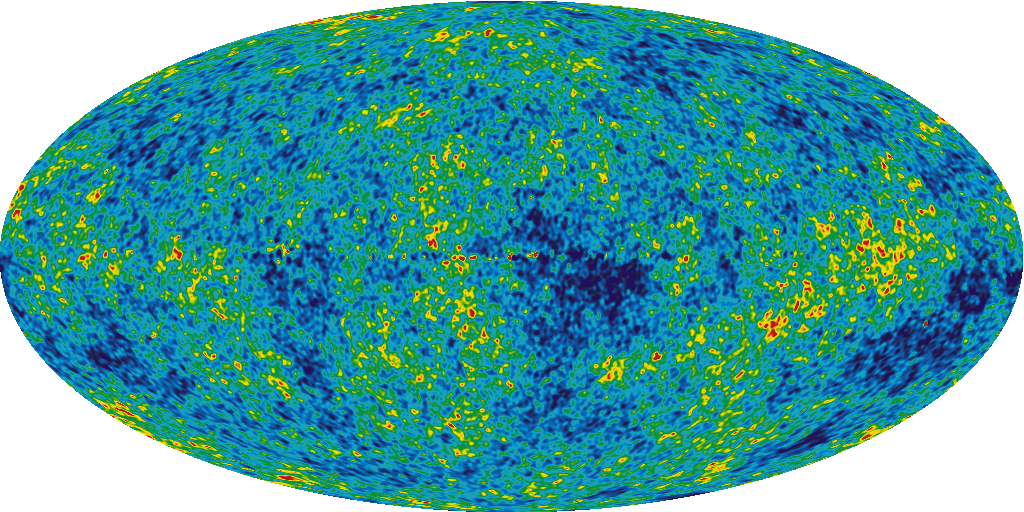
\includegraphics[width=0.7\textwidth]{cmb.png}
    \caption{\small CMBの異方性の観測は，初期宇宙が完全には一様でなかったことを示している．
    一方，その非一様性が小さく，一様な背景の周りの線形摂動として解析できることも観測からわかる．} % (see Figures \ref{fig:WMAP2} and \ref{fig:CMBparam}).}
    \label{fig:cmb}
\end{figure} 



\sectionlink{{\sl 復習}：宇宙論的摂動}

本講では，インフレーション中の量子揺らぎから宇宙論的摂動が生成される過程を詳しく示す．
この議論には宇宙論的摂動論の予備知識が必要なので，ここで簡単に復習する．
さらに詳しい説明は付録Aにある．
%In this section we give a general summary of cosmological perturbation theory. % \cite{Brandenberger:1993zc, Kodama:1985bj, Malik:2008im}. 
%In Section \ref{sec:qf} we then describe how these fluctuations arise as quantum fluctuations during the inflationary epoch.


%\subsectionlink{Linear Theory}





\subsectionlink{一般的事項}

\subsubsection{線形摂動}
CMBの観測（図\ref{fig:cmb}）は，宇宙論的摂動論が成功する理由を教えてくれる．
脱結合の時代の宇宙はほぼ一様で，非一様性は$10^{-5}$程度と小さかった．
したがって自然な方針は，すべての量$X(t, {\bf x})$（計量$g_{\mu \nu}$および物質場$T_{\mu \nu}$ $\to$ $\phi$ $\rho$, $p$など）を，宇宙時刻だけに依存する一様な背景$\bar X(t)$と，空間に依存する摂動とに分けることである．
\beq
\label{equ:pert}
\delta X(t, {\bf x}) \equiv X(t, {\bf x}) - \bar X(t)\, .
\eeq
摂動は小さいので，$\delta X \ll \bar X$，アインシュタイン方程式を摂動の線形次数まで展開すると，完全な非線形解を非常によい精度で近似できる．
\beq
\delta G_{\mu \nu} = 8\pi G\, \delta T_{\mu \nu}\, .
\eeq



\subsubsection{ゲージの選択}
宇宙論的摂動を調べる際の重要で微妙な点は，式(\ref{equ:pert})の背景と摂動への分割が一意ではなく，座標の選択，すなわち{\it ゲージの選択}に依存することである．\footnote{テンソル場$X$で表される任意の量の摂動$\delta X$は，物理的時空（摂動を受けた時空）での$X$の値と，与えられた（摂動のない）背景時空での同じ量の値$X_0$との差として定義される．しかし，テンソルの比較を意味のあるものとするには，この二つの異なる時空の点を同一視する処方が与えられてからでなければ比較できない，というのが微分幾何学の基本的な事実である．{\it ゲージの選択}とはまさにこのこと，すなわち背景時空と物理的時空の間の一対一の対応（写像）を与えることである．この写像の変更がゲージ変換であり，その選択の自由度によって，$X$がゲージ不変でない限り，任意の時空点における$X$の摂動の値には任意性が生じる．}
{\bf 第1講}で一様な宇宙を記述した際には，座標$t$と${\bf x}$を導入してFRW計量を定義した．
時刻$t$が一定の空間的超曲面が4次元時空の{\it スライシング}を定め，一方，${\bf x}$が一定の時間的世界線が{\it スレッディング}を定めた．
FRWのスレッディングは，自分の位置で運動量密度がゼロとなる共動観測者の運動に対応する．この観測者は自由落下し，彼らが定義する膨張は等方的である．スライシングはスレッディングに直交し，それぞれの空間的切片が一様な宇宙に対応する．
これらの特徴により，この座標の選択は際立って特別なものとなり，他の座標（そこでは宇宙が一様・等方には見えない）を気にする必要はなかった．
しかし，摂動を考える今は，摂動を受けた時空のスライシングとスレッディングが一意ではないことを認識するのが重要である．さらに，非一様な時空を記述する際には，特に好ましい座標の選び方が存在しないことも多い．
時空のスライシングとスレッディングを定めるためにゲージを選ぶと，暗黙のうちに摂動も定義している．
注意しないと，この摂動のゲージ依存性は混乱を招きうる．
このことを最も鮮明に示すため，エネルギー密度が時刻だけの関数$\rho(t, {\bf x})= \rho(t)$である，{\it 摂動のない}一様・等方な宇宙を考えよう．
ここで，時間座標の変更が{\it 見かけの}摂動$\delta \rho$を導入しうることを示す．新しい時間座標$\tilde t = t + \delta t(t, {\bf x})$を考える．一般に，新しい時間切片上ではエネルギー密度は一様ではなく，$\tilde \rho(\tilde t, {\bf x})= \rho(t(\tilde t, {\bf x}))$となる．このエネルギー密度の摂動は物理的なものではなく，すべて新しい時間スライシングの選択による．
同様に，時刻一定の超曲面をエネルギー密度一定の超曲面に一致させて選ぶと，エネルギー密度の{\it 実際の}摂動を取り除ける．このとき，実際に非一様性が存在していても$\delta \tilde \rho=0$となる．
一般相対論における実際の摂動と見かけの摂動の曖昧さを解消するには，摂動の完全な組を考える必要がある．すなわち，物質場の摂動と計量の摂動を両方考える必要があり，ゲージ変換によって一方を他方へ移し替えられる．
見かけのゲージモードの誤解を避けるには，摂動のゲージ不変な組合せを調べることも有用である．定義から，ゲージ不変量の揺らぎは座標変換で取り除けない．


\subsubsection{スカラー，ベクトル，テンソル}
空間的に平坦で一様・等方な背景時空は，多くの対称性をもつ．この対称性によって，計量とエネルギー運動量の摂動を
%associated with $\phi$ 
独立なスカラー（S），ベクトル（V），テンソル（T）成分に分解できる．この{\it SVT分解}はフーリエ空間で最も簡単に記述できる．
\beq
 X_{\bf k}(t) = \int \d^3 {\bf x} \  X(t, {\bf x}) \, e^{i {\bf k} \cdot {\bf x}}\, , \qquad X \equiv \delta \phi,\, \delta g_{\mu \nu}, \text{など}\, .
\eeq 摂動に対する線形運動方程式の{\it 並進不変性}は，異なるフーリエモードが相互作用しないことを意味する点に注意しよう（証明は付録\ref{sec:CPT}参照）．
したがって，異なるフーリエモードは独立に調べられる．これにより，摂動の微分方程式が簡単になることが多い．
次に，一つのフーリエ波数ベクトル${\bf k}$の周りの回転を考える．座標系を波数ベクトルの周りに角度$\psi$だけ回転したとき，その振幅に$e^{i m \psi}$が掛かる摂動は，ヘリシティ$m$をもつという．
\beq X_{\bf k} \to e^{im \psi} X_{\bf k}\, .
\eeq スカラー，ベクトル，テンソル摂動のヘリシティは，それぞれ$0$，$\pm 1$，$\pm 2$である．\footnote{ヘリシティによるこの抽象的なスカラー，ベクトル，テンソル摂動の定義がわかりにくければ，次節で導入する具体的な計量およびエネルギー運動量の摂動について，これらの規則を確かめてみるとよい．}SVT分解の重要な点は，それぞれの種類の摂動が（線形の範囲では）独立に時間発展し，したがって別々に扱えることである（証明は付録\ref{sec:CPT}参照）．
これにより，宇宙論的摂動の解析は大幅に簡単になる．

\vskip 8pt
以上の一般的な説明を踏まえ，さらに具体的に，一様・等方なFRW宇宙の周りの摂動を明示的に定義しよう．

%\subsectionlink{Metric and Stress-Energy Perturbations}

\subsectionlink{非一様な宇宙}

\subsubsection{計量摂動}
インフレーション中には，インフラトン$\bar \phi(t)$と計量$\bar g_{\mu \nu}(t)$の一様な背景解の周りで摂動を定義する．
\beq \phi(t, {\bf x}) = \bar \phi(t)
+ \delta \phi(t, {\bf x})\, , \qquad g_{\mu \nu}(t, {\bf x}) = \bar g_{\mu \nu}(t) + \delta g_{\mu \nu}(t, {\bf
x})\, , \eeq 
ここで，
\bea
\d s^2 &=& g_{\mu \nu}\, \d x^\mu \d x^\nu \nonumber \\
&=& -(1+2 \Phi) \d t^2 + 2 a B_i \d x^i \d t + a^2 [(1-2 \Psi) \delta_{ij} + E_{ij}] \d x^i \d x^j\, .
\label{equ:perturbed} 
\eea
実空間での計量摂動(\ref{equ:perturbed})のSVT分解は次のようになる．\footnote{実空間でのSVT分解は，空間的超曲面上でのスカラー，ベクトル，テンソルの異なる変換性に対応する．}
\beq \label{equ:SVT1} B_i \equiv
\partial_i B- S_i\, , \qquad \text{ただし} \quad  \partial^i S_i = 0\, , \eeq また，\beq \label{equ:SVT2}
 E_{ij} \equiv 2 \partial_{ij} E + 2 \partial_{(i} F_{j)} + h_{ij}\, ,  \qquad \text{ただし} \quad \partial^i F_i =0\, , \quad h^i_{i} = \partial^i h_{ij} = 0\, .
\eeq
ベクトル摂動$S_i$と$F_i$はインフレーションでは生成されない（いずれにせよ宇宙の膨張とともに減衰する）．この理由から，本講義ではベクトル摂動を無視する．
以下では，後期宇宙で密度揺らぎと重力波として観測されるスカラー揺らぎとテンソル揺らぎに注目する．

テンソル揺らぎはゲージ不変だが，スカラー揺らぎは座標の変更に伴って変化する．
次のゲージ変換を考える．
\bea
t &\to& t + \alpha \\
x^i &\to& x^i + \delta^{ij} \beta_{,j}\, .
\eea
この座標変換の下で，スカラー計量摂動は次のように変換される．
\bea
\Phi &\to& \Phi - \dot \alpha\label{equ:d1} \\
B &\to& B + a^{-1} \alpha - a \dot \beta \\
E &\to& E - \beta \\
\Psi &\to& \Psi + H \alpha\, . \label{equ:d2}
\eea

\begin{thm}[線形ゲージ変換]
スカラー計量摂動のゲージ変換(\ref{equ:d1})--(\ref{equ:d2})を導け．ヒント：時空間隔の不変性を用いよ．
\beq
\d s^2 = g_{\mu \nu} \d x^\mu \d x^\nu = \tilde g_{\mu \nu} \d \tilde x^\mu \d \tilde x^\nu\, .
\eeq
\label{ex:gauge}
\end{thm}

\subsubsection{物質摂動}
インフレーション中には，インフレーションのエネルギーが宇宙のエネルギー運動量への支配的な寄与を与えるため，インフラトンの摂動$\delta \phi$は時空幾何に逆反応する．
この物質摂動と計量摂動の結合は，アインシュタイン方程式によって記述される（付録\ref{sec:CPT}参照）．

インフレーション後，宇宙の全エネルギー運動量テンソルの摂動は次のようになる．
\bea
T^0_0 &=& - (\bar \rho + \delta \rho) \\
T^0_i &=& (\bar \rho +\bar p)\, av_i \\
T^i_0 &=& -(\bar \rho + \bar p) (v^i - B^i)/a \\
T^i_j &=& \delta^i_j (\bar p + \delta p) + \Sigma^i_j\, .
\eea
異方性応力$\Sigma^i_j$はゲージ不変である一方，密度，圧力，運動量密度（$(\delta q)_{,i} \equiv (\bar \rho + \bar p) v_i$）は次のように変換される．
\bea
\delta \rho &\to& \delta \rho - \dot {\bar \rho} \,\alpha \\
\delta p &\to& \delta p - \dot {\bar p}\, \alpha \\
\delta q &\to& \delta q + (\bar \rho + \bar p)\, \alpha\, .
\eea



\subsubsection{ゲージ不変変数}

上で説明したように，見かけのゲージモードという落とし穴を避けるには，計量摂動と物質摂動のゲージ不変な組合せを導入すると便利である\cite{Bardeen:1980kt}．
重要なゲージ不変スカラー量の一つは，{\it 一様密度超曲面上の曲率摂動}である\cite{BST}．
\beq
\fbox{$\displaystyle
\label{equ:zeta} - \zeta \equiv  \Psi +  \frac{H}{\dot{\bar \rho}}
\delta \rho $} \, .
\eeq
%where $\rho$ is the total energy density of the universe.
幾何学的には，$\zeta$は密度一定の超曲面の空間曲率$R^{(3)} = 4 \nabla^2 \Psi/a^2$を測る．$\zeta$の重要な性質は，断熱的な物質摂動，すなわち次式を満たす摂動に対して，地平線の外側で一定にとどまることである．
\beq
\label{equ:ad:source-duplicate-1}
\fbox{$\displaystyle
\delta p_{en} \equiv \delta p - \frac{\dot {\bar p}}{\dot {\bar \rho}} \delta \rho $} = 0\, .
\eeq
$\delta p_{en}$の定義がゲージ不変であることに注意しよう．
本講で扱う単一場インフレーション模型では条件(\ref{equ:ad})が常に満たされるので，摂動$\zeta_{\bf k}$は地平線の外側$k \ll aH$では時間発展しない．


空間的に平坦な超曲面$\Psi$で定義されるゲージでは，摂動$\zeta$は無次元の密度摂動$\frac{1}{3} \delta \rho/(\bar \rho+ \bar p )$である．
%On sub-horizon scales $\zeta$ is related to density perturbations $\delta \rho$.
したがって，地平線内での揺らぎの時間発展を記述する適切な伝達関数を考慮すると，CMBおよび大規模構造（LSS）の観測を$\zeta$の原始的な値に結び付けられる（{\bf 第3講}参照）．
スローロール・インフレーション中には，
\beq
\label{equ:zetaSR}
- \zeta \approx \Psi + \frac{H}{\dot{\bar \phi}} \delta \phi\, .
\eeq

もう一つのゲージ不変スカラーは{\it 共動曲率摂動}である．
\beq
\fbox{$\displaystyle
{\cal R} \equiv \Psi - \frac{H}{\bar \rho + \bar p} \delta q $}\, ,
\eeq
ここで，$\delta q$は3次元運動量密度$T^0_i = \partial_i \delta q$のスカラー部分である．
インフレーション中には$T^0_i = - \dot{\bar \phi}\, \partial_i \delta \phi$なので，
\beq
\label{equ:RSR}
\R = \Psi + \frac{H}{\dot{\bar \phi}} \delta \phi\, .
\eeq
幾何学的には，${\cal R}$は共動超曲面（または$\phi$一定の超曲面）の空間曲率を測る．%, $R^{(3)} = -4 \nabla^2 {\cal R}/a^2$.

線形化したアインシュタイン方程式は，$\zeta$と${\cal R}$を次のように関係付ける（付録\ref{sec:CPT}参照）．
\beq
-\zeta = {\cal R} + \frac{k^2}{(aH)^2} \frac{2 \bar \rho}{3(\bar \rho + \bar p)} \Psi_{\rm B}\, ,
\eeq
ここで，
\beq
\Psi_{\rm B} \equiv \psi + a^2 H (\dot E - B/a)\, ,
\eeq
はバーディーン・ポテンシャルの一つである\cite{Bardeen:1980kt}．
したがって，$\zeta$と${\cal R}$は地平線より大きなスケール$k \ll aH$で等しい．
また，$\zeta$と${\cal R}$はスローロール・インフレーション中にも等しい．式(\ref{equ:zetaSR})と(\ref{equ:RSR})を参照．
したがって，$\zeta$と$\R$の相関関数は地平線通過時に等しく，$\zeta$と$\R$はいずれも地平線より大きなスケールで保存される．
本講では，地平線通過時の$\R$の原始スペクトルを計算する．

最後に，インフラトン摂動のゲージ不変な尺度は，{\it 空間的に平坦な切片上のインフラトン摂動}である．
\beq
\fbox{$\displaystyle
Q \equiv \delta \phi + \frac{\dot {\bar \phi}}{H}\Psi $}\, .
\eeq

\begin{thm}[ゲージ不変な摂動]
計量摂動と物質摂動の線形ゲージ変換を用い，$\zeta$，$\R$，$Q$がゲージ不変であることを確かめよ．
\label{ex:gauge2}
\end{thm}


\subsubsection{地平線より大きなスケールでの時間発展（とその不在）}


アインシュタイン方程式（付録\ref{sec:CPT}参照）は，ゲージ不変な曲率摂動に対して次の時間発展方程式を与える．
\beq
\dot \R = -  \frac{H}{\bar \rho + \bar p}\, \delta p_{en} + \frac{k^2}{(aH)^2} \Bigl(\dots \Bigr)\, .
\eeq
断熱的な物質摂動は$\delta p_{en} =0$を満たし，$\R$は地平線より大きなスケール$k < aH$で保存される．

\begin{thm}[別個の宇宙のアプローチ]
地平線より大きなスケールにおける曲率摂動$\R$の保存を証明する，別個の宇宙のアプローチ\cite{Wands:2000dp}について読め．
\label{ex:separate:source-duplicate-1}
\end{thm}


\subsectionlink{宇宙論的摂動の統計}


原始スカラー揺らぎの重要な統計的尺度は，$\R$（または$\zeta$）のパワースペクトルである．\footnote{無次元パワースペクトル$\Delta_\R^2(k)$の規格化は，$\R$の分散が$\langle \R \R \rangle = \int_0^\infty \Delta_\R^2(k) \, \d \ln k$となるように選んでいる．}
\beq \langle \R_{\bf k} \R_{{\bf k}'}
\rangle = (2\pi)^3 \, \delta({\bf k} + {\bf k}') \, P_\R(k)\, , \qquad \Delta_{\rm s}^2 \equiv \Delta_\R^2 = \frac{k^3}{2\pi^2} P_\R(k)\, .  \eeq
%\beq \langle \zeta_{\bf k} \zeta_{{\bf
%k}'} \rangle = (2\pi)^3 \delta({\bf k} + {\bf k}') {\cal P}_s(k)\, , \qquad P_s(k) \equiv \frac{k^3}{2 \pi^2}
%{\cal P}_s(k) \eeq
ここで，$\langle \, ...\, \rangle$は揺らぎのアンサンブル平均を表す．
パワースペクトルのスケール依存性は，スカラー・スペクトル指数（または傾き）によって定義される．\beq
\label{equ:ns}
n_{\rm s} - 1 \equiv \frac{d
\ln \Delta^2_{\rm s}}{d \ln k}\, ,\eeq
ここで，スケール不変性は$n_{\rm s} = 1$に対応する．スペクトル指数のランニングも次のように定義できる．\beq \label{equ:as}
 \alpha_{\rm s}
\equiv \frac{d n_{\rm s}}{d \ln k}\, . \eeq
パワースペクトルは，しばしば次のべき乗則の形で近似される．
\beq
\Delta_{\rm s}^2(k) = A_{\rm s}(k_\star) \left(\frac{k}{k_\star}\right)^{n_{\rm s}(k_\star)-1+ \frac{1}{2} \alpha_{\rm s}(k_\star) \ln (k/k_\star)}\, ,
\eeq
ここで，$k_\star$は任意の基準スケール，またはピボットスケールである．

$\R$がガウス的なら，パワースペクトルはすべての統計的情報を含む．原始非ガウス性は，$\R$の高次相関関数に符号化されている．
%(see \S\ref{sec:NG}).
単一場スローロール・インフレーションでは，非ガウス性は小さいと予言される\cite{Acquaviva02,malda}．
しかし，多場模型や，非自明な運動項をもつ，あるいはスローロール条件を破る単一場模型では，非ガウス性が大きくなることがある．
原始非ガウス性には{\bf 第4講}で戻る．本講では，計算をガウス揺らぎとそれに伴うパワースペクトルに限る．


$h_{ij}$の二つの偏極モード，すなわち$h \equiv h^+, h^\times$のパワースペクトルは次のように定義される．\beq \langle h_{\bf k} h_{{\bf k}'} \rangle = (2\pi)^3\, \delta({\bf
k} + {\bf k}')\, P_h(k)\, , \qquad \Delta_h^2 = \frac{k^3}{2\pi^2} P_h(k)\, .  %\qquad P_t(k) \equiv \frac{k^3}{2 \pi^2} {\cal P}_t(k)
\eeq
テンソル摂動のパワースペクトルを，二つの偏極のパワースペクトルの和として定義する．
\beq
\Delta_{\rm t}^2 \equiv 2 \Delta_h^2\, .
\eeq
そのスケール依存性は式(\ref{equ:ns})と同様に定義されるが，歴史的理由から$-1$を付けない．
\beq n_{\rm t} \equiv \frac{d \ln \Delta^2_{\rm t}}{d \ln k}\, , \eeq
すなわち，
\beq
\Delta^2_{\rm t}(k) = A_{\rm t}(k_\star) \left(\frac{k}{k_\star}\right)^{n_{\rm t}(k_\star)}\, .
\eeq

%CMB polarization measurements are sensitive to the ratio of tensor  power to scalar power \beq r \equiv \frac{P_t}{P_s}  \, . \eeq The parameter $r$ will be of fundamental
%importance for the discussion presented in this paper.
%As we argue in Section \ref{sec:Bmodes}, its value encodes crucial information about the physics
%of the inflationary era.

\vspace{0.5cm}
%\underline{\bf Aim of this lecture:} 
\subsubsection*{本講の目的}
本講の目的は，スカラー揺らぎとテンソル揺らぎのパワースペクトル$P_\R(k)$と$P_h(k)$を第一原理から計算することである．
これは現代の理論宇宙論において最も重要な計算の一つであり，理解するために努力する価値は十分にある．

%\subsectionlink{Three Gauges and $\zeta$, ${\cal R}$ and $Q$}

%\subsubsection{Uniform Density Gauge}

%define $\zeta$

%\subsubsection{Comoving Gauge}

%define ${\cal R}$

%\subsubsection{Spatially-Flat Gauge}

%define $Q$

 
%\newpage
%%%%%%%%%%%%%%%%%%%%%%%%%%%%%%%%%%
\sectionlink{{\sl 概観}：構造の量子的起源} %: A Qualitative (Pre)View}
%\sectionlink{Quantum Fluctuations as the Origin of Structure}
\label{sec:qf}
%%%%%%%%%%%%%%%%%%%%%%%%%%%%%%%%%%

%{\tt more. add some things fro Will's intro}\\


前講では，インフラトン場の古典的な時間発展を論じた．インフラトンの量子揺らぎを考えると，驚くべきことが起こる．インフレーションと量子力学を組み合わせると，宇宙のあらゆる構造の初期の種を生成する美しい機構が得られるのである．言い換えると，インフレーション中の量子揺らぎが，スカラー揺らぎとテンソル揺らぎの原始パワースペクトル$P_{\rm s}(k)$と$P_{\rm t}(k)$の源となる．
本節では，インフレーションが微視的な物理を巨視的な観測量に結び付ける機構を概説する．
\S\ref{sec:full}では完全な計算を示す．


\begin{figure}[htbp]
    \centering
        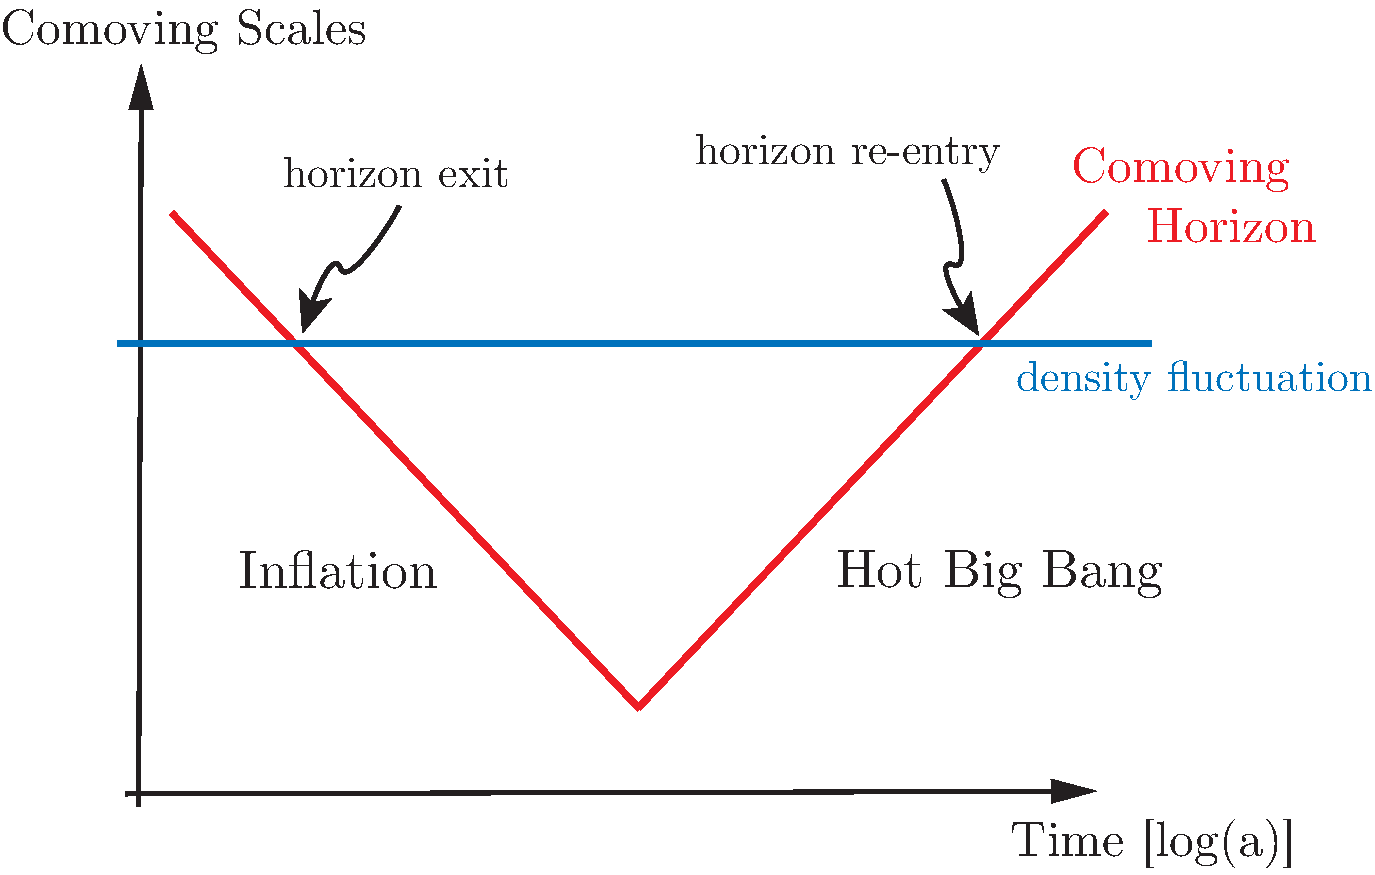
\includegraphics[width=0.65\textwidth]{./Scales}
   \caption{\small インフレーション宇宙における摂動の生成と時間発展．揺らぎは地平線内のスケールで量子力学的に生成される．共動スケール$k^{-1}$が一定に保たれる一方，インフレーション中の共動ハッブル半径$(aH)^{-1}$は縮小し，摂動は地平線の外へ出る．因果的な物理過程は地平線より大きな摂動に作用できず，摂動は後の時代に地平線へ再突入するまで凍結する．}
    \label{fig:scales}
\end{figure}

\subsectionlink{量子的な零点揺らぎ}

\S\ref{sec:full}で定量的に説明するように，インフレーション中の量子揺らぎは，すべての軽い場（インフラトンや計量摂動など）の揺らぎにゼロでない分散を生じさせる．
これは，基底状態での零点揺らぎが調和振動子の振幅に生む分散と非常によく似ている．\S\ref{sec:SHO}参照．
揺らぎの振幅は，インフレーション中の膨張パラメータ$H$に比例する．
これはド・ジッター地平線$H^{-1}$に関係しており，インフレーション中の量子揺らぎは，ブラックホールのホーキング放射との密接な類似の下で，ド・ジッター空間の熱揺らぎとして解釈することもできる．

揺らぎはすべての長さスケールで，すなわち波数$k$のスペクトルをもって生成される．
宇宙論的に重要な揺らぎは，地平線（ハッブル半径）の内側で生まれる．
\beq \text{地平線内：} \quad
k \gg aH\, .
\eeq
しかし，共動波数が一定である一方，共動ハッブル半径はインフレーション中に縮小する（これがインフレーションの「定義」であったことを思い出そう）．したがって，やがてすべての揺らぎは{\it 地平線の外へ出る}．
\beq \text{地平線外：} \quad
k < aH\, .
\eeq

\subsectionlink{地平線からの退出と再突入}

宇宙論的な非一様性は，物質に関して定義した空間的超曲面の内在的曲率$\R$または$\zeta$によって特徴付けられる．
${\cal R}$と$\zeta$はどちらも，地平線の外側，すなわち$k < aH$で一定にとどまるという便利な性質をもつ．
特に，その振幅はインフレーション直後の宇宙の未知の物理的性質の影響を{\it 受けない}（再加熱の詳細についてはほとんど何もわかっていないことを思い出そう．それでも宇宙論的観測量を予言できるのは，地平線の外側で$\R$と$\zeta$が一定であるためである）．
インフレーション後には共動地平線が成長するので，やがてすべての揺らぎは地平線へ再突入する．
地平線再突入後，$\R$または$\zeta$は宇宙流体の摂動を定め，観測されるCMB異方性とLSSをもたらす．\\ % (see Lecture 3).\\


%\subsectionlink{The Physical Importance of ${\cal R}$ and $\zeta$}


{\bf 第1講}では，インフレーション中と，その後の標準的なFRW膨張中における共動地平線の時間発展を説明した．
本講（{\bf 第2講}）では，地平線退出時の共動曲率揺らぎ$\R$の原始パワースペクトルを計算する．
次講（{\bf 第3講}）では，曲率揺らぎ$\R$と，地平線再突入後の宇宙論的観測量の揺らぎとの関係を計算する．
したがって，この三つの講義を合わせると，インフレーションが生成する量子揺らぎの生成過程と観測への帰結の両方について，完全な説明が得られる．
これは美しい物語である．その展開を始めよう．

\sectionlink{調和振動子の量子力学} %Simple
\label{sec:SHO}

\begin{quote}
「若い理論物理学者の歩みは，抽象度をますます高めながら調和振動子を扱うことからなる．」

{\it Sidney Coleman}
\end{quote}

%Since inflation stretches microscopic scales into astronomical ones, it suggests the possibility that the density perturbations which provide the seeds for galaxy formation might have originated as microscopic quantum fluctuations.
インフレーション中に生成される量子揺らぎの計算は，代数計算がかなり多い．そこで，関係する物理の大部分を含みつつ，より簡単な例から始めるのが有益である．準備として，1次元の単純調和振動子の量子化を考えよう．
調和振動子は，物理学者が厳密に解ける数少ない物理系の一つである．幸い，もっと複雑な物理系もほぼすべて，振幅と振動数の異なる単純調和振動子の集まりとして表現できる．
% (remember normal modes in classical dynamics?). 
これはもちろん，フーリエ解析そのものである．
以下では，曲がった時空（特にド・ジッター空間）における自由場が，時間に依存する振動数をもつ調和振動子の集まりに似ていることを示す．したがって，本節で量子調和振動子を詳しく扱うことは無駄ではなく，インフレーションの計算に重要な直観を与える．本節は文献\cite{Jacobson:2003vx}の優れた解説に基づく．

\subsectionlink{作用}

時間に依存する振動数をもつ調和振動子の古典作用は，
\begin{equation}
S = \int \d t \, \left(\frac{1}{2} \dot{x}^2 -\frac{1}{2} \omega^2(t) x^2 \right) \equiv \int \d t \, L\, ,
\end{equation}
ここで，$x$は平衡状態$x \equiv 0$からの粒子のずれであり，便宜上，粒子の質量を1，$m \equiv 1$とした．具体的には，外部の熱源によって加熱され，ばね定数$k(t)$が時間に依存するばねにつながれた質量$m$の粒子を考えるとよい．ただし$\omega^2 =k/m$である．古典的な運動方程式は，粒子座標$x$に関する作用の変分から得られる．
\begin{equation}
\frac{\delta S}{\delta x} = 0 \quad \Rightarrow \quad \fbox{$\displaystyle \ddot{x} + \omega^2(t)\, x =0 $}\, .
\end{equation}

\subsectionlink{正準量子化}
系の正準量子化は標準的な手順で行う．
$x$に共役な運動量を定義する．
\begin{equation}
p \equiv \frac{d L}{d \dot{x}} = \dot{x},
\end{equation}
これは粒子の運動量の通常の定義$p=mv$と一致する．
次に，古典変数$x$，$p$を量子演算子$\hat{x}$，$\hat{p}$に昇格させ，正準交換関係を課す．
\begin{equation}
\label{equ:commutator}
\fbox{$\displaystyle
\left[\hat{x}, \hat{p} \right] = i \hbar $}\, ,
\end{equation}
ここで，$[\hat x, \hat p] \equiv \hat x \hat p - \hat p \hat x$である．
運動方程式によれば，この交換関係をある初期時刻に課すと，すべての時刻で成り立つ．特に，現在の例では，
\begin{equation}
\left[x(t), \dot{x}(t) \right] = i \hbar\, .
\end{equation}
ここでは演算子が時間変化し，状態は時間に依存しないハイゼンベルク描像を用いていることに注意しよう．
演算子$\hat x$を生成・消滅演算子で展開する．
\begin{equation}
\fbox{$\displaystyle
\hat{x} = v(t) \, \hat{a} + v^*(t) \, \hat{a}^\dagger $}\, ,
\end{equation}
ここで，（複素）モード関数は古典的な運動方程式を満たす．
\begin{equation}
\label{equ:veqn}
\ddot{v}+\omega^2(t) v =0\, .
\end{equation}
交換関係(\ref{equ:commutator})は次のようになる．
\begin{equation}
\langle v,v \rangle [\hat{a}, \hat{a}^\dagger ]= 1\, ,
\end{equation}
ここで，
\begin{equation}
\langle v,w \rangle \equiv \frac{i}{\hbar} \left(v^* \partial_t w - (\partial_t v^*) w \right)\, .
\end{equation}
一般性を失わずに，実数$\langle v,v \rangle$が正となるように解$v$を選んだとする．すると，関数$v$を再スケールして$\langle v,v \rangle \equiv 1$とできるので，
\begin{equation}
\label{equ:aa}
\fbox{$\displaystyle [\hat{a}, \hat{a}^\dagger ]=1$}\, .
\end{equation}
式(\ref{equ:aa})は，調和振動子の昇降演算子の標準的な関係式である．
したがって，次の消滅・生成演算子を同定した．
\begin{eqnarray}
\hat{a} &=& \langle v, \hat{x} \rangle\\
\hat{a}^\dagger &=& -\langle v^*, \hat{x} \rangle\, ,
\end{eqnarray} 
また，真空状態$| 0 \rangle$を次の処方で定義できる．
\begin{equation}
\fbox{$\displaystyle \hat{a} | 0 \rangle = 0$}\, ,
\end{equation}
すなわち，真空は$\hat a$によって消される．
系の励起状態は，生成演算子を繰り返し作用させて作る．
\begin{equation}
| n \rangle \equiv \frac{1}{\sqrt{n!}} (\hat{a}^\dagger)^n | 0 \rangle\, .
\end{equation}
これらの状態は，数演算子$\hat{N} = \hat{a}^\dagger \hat{a}$の固有値$n$の固有状態である．すなわち，
\beq
\hat N | n \rangle = n | n \rangle\, .
\eeq


\subsectionlink{モード関数の非一意性}

まだモード関数を一意に定めていないため，真空状態も確定していない．
解$x(t)$を変えない$v(t)$の任意の変更は，演算子$\hat{a} = \langle v, \hat{x}\rangle$の変更，したがって真空の定義の変更をもたらす．
時間に依存する振動数$\omega(t)$をもつ単純調和振動子（および曲がった時空における量子場）では，実際，モード関数$v(t)$の一意な選択は{\it 存在しない}．したがって，$\hat{x}$の生成・消滅演算子への一意な分解も，真空の一意な概念も{\it 存在しない}．解$v(t)$の選び方が異なれば，異なる真空解が得られる．この問題と，インフレーションの場合の標準的な（ただし異論のないわけではない）解決法については，以下でさらに詳しく論じる．

%{\it Special case of constant frequency $\omega(t) = \omega$}. 

\vskip 6pt
ここでは，振動数が一定の調和振動子$\omega(t) =\omega$という特別な場合を考えると先に進める．\footnote{これは，すべてのモードが地平線の十分内側にある非常に初期のインフレーションに関係する場合であることがわかる．}この場合，真空状態$|0\rangle$をハミルトニアンの基底状態にする$v(t)$の選択が好ましい．
まず，一般のモード関数$v(t)$についてハミルトニアンを計算する．
\begin{eqnarray}
\hat{H} &=& \frac{1}{2} \hat{p}^2 +\frac{1}{2} \omega^2 \hat{x}^2 \\
&=& \frac{1}{2} \left[(\dot{v}^2 + \omega^2 v^2) \hat{a} \hat{a}  + (\dot{v}^2 + \omega^2 v^2)^* \, \hat{a}^\dagger \hat{a}^\dagger +(|\dot{v}|^2 +\omega^2 |v|^2) (\hat{a}\hat{a}^\dagger + \hat{a}^\dagger \hat{a})\right]\nonumber\, .
\end{eqnarray} 
$\hat{a} |0\rangle =0$と$[\hat{a},\hat{a}^\dagger]=1$を用いると，ハミルトニアン演算子の真空状態への作用は次のようになる．
\begin{equation}
\hat{H} |0 \rangle = \frac{1}{2} (\dot{v}^2 + \omega^2 v^2)^*\, \hat{a}^\dagger \hat{a}^\dagger |0 \rangle + \frac{1}{2}(|\dot{v}|^2 +\omega^2 |v|^2) |0 \rangle\, . 
\end{equation}
$|0\rangle$が$\hat{H}$の固有状態であるという要請は，第1項が消えなければならないことを意味し，次の条件を与える．
\begin{equation}
\label{equ:modes}
\dot{v} = \pm i \omega v\, ,
\end{equation}
したがって，
\begin{equation}
\langle v, v \rangle = \mp \frac{2 \omega}{\hbar} |v|^2\, .
\end{equation}
規格化条件の正値性$\langle v, v \rangle > 0$は，式(\ref{equ:modes})の負符号を選ぶ．
\begin{equation}
\dot{v} = - i \omega v\, .
\end{equation}
適切に規格化（$\langle v, v \rangle = 1$）すると，次の{\it 正振動数解}が得られる．
\begin{equation}
\label{equ:mode2}
\fbox{$\displaystyle v(t) = \sqrt{\frac{\hbar}{2 \omega}} \, e^{-i \omega t}$}\, .
\end{equation}
モード関数$v$をこのように選ぶと，ハミルトニアンは，
\begin{equation}
\hat{H} = \hbar \omega \left(\hat{N}+\frac{1}{2} \right)\, ,
\end{equation}
このハミルトニアンに対して，真空$|0\rangle$は最低エネルギー$\hbar \omega /2$の状態である．
%If any function other than (\ref{equ:mode2}) is chosen to expand the position operator, then the state annihilated by $\hat{a}$ is {\it not} the ground state of the oscillator.\\

\begin{thm}[時間依存振動子の非一意性]
振動数が時間に依存する単純調和振動子の場合，上の議論のどこが成り立たなくなるか．
\label{ex:separate}
\end{thm}

\subsectionlink{基底状態の零点揺らぎ}

基底状態$|0\rangle$における位置演算子$\hat{x}$の二乗平均の期待値を考える．
\begin{eqnarray}
\langle |\hat{x}|^2 \rangle &\equiv& \langle 0|\hat{x}^\dagger \hat{x}|0\rangle \nonumber\\
&=& \langle 0|(v^* \hat{a}^\dagger + v \hat{a})(v \hat{a}+v^* \hat{a}^\dagger )|0\rangle \nonumber\\
&=& |v(\omega,t)|^2 \langle 0|\hat{a} \hat{a}^\dagger |0\rangle \nonumber\\
&=& |v(\omega,t)|^2 \langle 0|[\hat{a}, \hat{a}^\dagger] |0\rangle \nonumber\\
&=& |v(\omega,t)|^2\, .
\end{eqnarray}
これは，真空状態での位置の零点揺らぎをモード関数の絶対値の二乗で特徴付ける．
\begin{equation}
\label{equ:fluc}
\fbox{$\displaystyle \langle |\hat{x}|^2 \rangle = |v(\omega,t)|^2$} = \frac{\hbar}{2\omega}\, .
\end{equation}
インフレーションが生成する揺らぎのスペクトルを計算するために必要な量子力学の知識は，これですべてである．
ただし，その前に，宇宙論的摂動のスカラーモードに対するモード方程式，すなわち式(\ref{equ:veqn})に対応する方程式を導くため，かなりの作業が必要である．



\sectionlink{ド・ジッター空間の量子揺らぎ}
\label{sec:full}

ついに本講の見せ場に到達した．インフレーション中に生成される量子力学的揺らぎの完全な計算と，宇宙論的摂動との関係である．この計算はマルダセナの扱い\cite{malda}にほぼ沿って進める．


\subsectionlink{計算方針のまとめ}

直前の二つの節は退屈だったかもしれないが，インフレーションの揺らぎを計算するための重要な準備となった．
ゲージ不変な曲率摂動${\cal R}$を定義した．これは地平線の外側で保存されるので，地平線退出時に計算すれば，ある${\cal R}$モードが地平線へ再突入するまで，再加熱中およびその後の地平線内の物理を知らなくてもよい．
単純調和振動子の量子化も復習したので，${\cal R}$の運動方程式を単純調和振動子の形に書けば，インフレーション中のスカラー揺らぎの量子化を調べる準備が整う．\\

以下の各節で行う手順をまとめておく．

\begin{enumerate}
\item 単一場スローロール・インフレーションの作用を，揺らぎの2次まで展開する．
特に，${\cal R}$を用いた作用の2次展開を導く．
作用に基づく方法では，揺らぎの量子化における正しい規格化が保証される．
\item 作用から${\cal R}$の運動方程式を導き，単純調和振動子（SHO）の形になることを示す．
\item ${\cal R}$のモード方程式を厳密に解くことは難しいので，スローロールの時間発展中に有効な近似解をいくつか考える．
\item 古典場${\cal R}$を量子演算子に昇格させ，量子化する．
量子演算子に正準交換関係を課すと，モード関数に対する境界条件が得られる．ただし，これだけではモード関数は完全には定まらない．
\item 得られた解を紫外領域，すなわちモードが地平線の十分内側にある小さなスケールでミンコフスキー真空に接続し，真空状態を定義する．
これによりモード関数が完全に定まり，その大スケール極限も定まる．
\item 次に，地平線通過時の曲率揺らぎのパワースペクトルを計算する．{\bf 第3講}では，インフレーション中の地平線通過時のパワースペクトルを，再結合時のCMB揺らぎの角度パワースペクトルに関係付ける．
\end{enumerate}

\noindent
説明はこれくらいにして，計算を始めよう！

\subsectionlink{スカラー摂動}

次の作用で定義される単一場スローロール・インフレーション模型を考える．
\beq
\label{equ:SRaction1}
S = \frac{1}{2} \int \d^4 x \sqrt{-g}\, \left[R-(\nabla \phi)^2 - 2 V(\phi)
\right]\, , %\qquad \Mp^{-2} \equiv 8 \pi G = 1\, .
\eeq
単位系は$ \Mp^{-2} \equiv 8 \pi G = 1$とする．
時間と空間の再パラメータ化を固定するため，力学変数$g_{ij}$と$\phi$に対して次のゲージを選ぶ．
\beq
\delta \phi = 0\, , \qquad g_{ij} = a^2 [(1- 2 \R) \delta_{ij} + h_{ij}]\, , \qquad \partial_i h_{ij} = h^i_{i} = 0\, .
\eeq
このゲージでは，インフラトン場には摂動がなく，すべてのスカラー自由度は計量揺らぎ
%\footnote{As we explained above, the curvature perturbation in comoving gauge, $T^0_i=0$ ($\delta \phi=0$), is actually called ${\cal R}$, reserving $\zeta$ for the curvature perturbation in uniform density gauge. This mislabeling has become standard in the literature, so to facilitate comparison with results in other papers we here admit to committing this sin as well. In practice, the difference between ${\cal R}$ and $\zeta$ is unimportant since our aim is to compute their power spectra at horizon crossing where they are the same.}
%, since ${\cal R}$ and $\zeta$ are the same on superhorizon scales.} 
$\R(t, {\bf x})$でパラメータ化される．
$\R$の重要な性質は，地平線の外側で一定にとどまることである．したがって，計算を地平線通過時の$\R$の相関関数に限ることができる．
残りの計量摂動$\Phi$と$B$は，アインシュタイン方程式によって$\R$に関係付けられる．ADM形式（付録\ref{sec:malda}参照）では，これらは純粋な拘束方程式である．

\subsubsection{自由場の作用}

かなりの計算を行うと（付録\ref{sec:malda}参照），作用(\ref{equ:SRaction1})を$\R$の2次まで展開できる．
\beq
\label{equ:S(2)}
\fbox{$\displaystyle
S_{(2)} = \frac{1}{2} \int \d^4 x \, a^3 \frac{{\dot{\phi}}^2}{H^2} \left[ \dot \R^2 - a^{-2} (\partial_i \R)^2 \right]  $} \, .%\equiv \int \d \tau \d^3 x \, a^2 \, \epsilon \, \Box \zeta\, .
\eeq
{\it ムハノフ変数}を定義し，
\beq
v\equiv z \R \, , \qquad \text{ただし} \qquad z^2 \equiv a^2 \frac{{\dot{\phi}}^2}{H^2}= 2a^2 \varepsilon\, ,
\eeq
共形時刻$\tau$に移ると，正準規格化されたスカラーの作用が得られる．
\beq
\label{equ:S2v2}
\fbox{$\displaystyle
S_{(2)} =\frac{1}{2} \int \d \tau \d^3 x \ \left[ (v')^2 + (\partial_i v)^2  + \frac{z''}{z} v^2\right] $}\, , \qquad (...)' \equiv \partial_\tau(...)\, .
\eeq
%where
%\beq \Delta \equiv - \frac{\partial^2}{\partial \tau^2} + \partial^2 + \frac{z''}{z}\, . \eeq
\begin{thm}[ムハノフ作用]
式(\ref{equ:S2v2})を確かめよ．ヒント：部分積分を用いよ．
 \end{thm}
場$v$のフーリエ展開を
%\footnote{Note that the coordinates ${\bf x}$ are comoving coordinates, and the wavevector ${\bf k}$, which does not redshift with expansion. The proper wavevector is ${\bf k}_{\rm prop} = {\bf k}/a(\tau)$. Therefore, the comoving wavenumber ${\bf k}$ is not itself dynamical, but is just a set of constants labeling a particular Fourier component.} 
次のように定義する．
\beq
v(\tau, {\bf x}) = \int \frac{\d^3 k}{(2\pi)^3} \, v_{\bf k}(\tau) e^{i {\bf k} \cdot {\bf x}}\, ,
\eeq
ここで，
\beq
\label{equ:Mmode}
\fbox{$\displaystyle
v_k'' + \left( k^2 - \frac{z''}{z}\right) v_k = 0 $}\, .
\eeq
式(\ref{equ:Mmode})は$k$の大きさだけに依存するので，添字のベクトル表記${\bf k}$を省略した．
関数$z$が背景の力学に依存するため，ムハノフ方程式(\ref{equ:Mmode})を完全に一般的な形で解くことは難しい．
インフレーションの背景が与えられれば，式(\ref{equ:Mmode})を数値的に解ける．
しかし，解をより直観的に理解するため，純粋なド・ジッター極限（\S\ref{sec:dSmode}）とスローロール近似（{\bf 問題\ref{ex:SRmode}}）における近似解析解を論じる．
%where
%$\nu^2$ is a combination of terms that are linear and quadratic in the slow-roll parameters (however, {\it no} slow-roll approximation has been made. So far this is exact.).

%\beq
%\nu \approx \frac{3}{2} + 3 \epsilon - \eta
%\eeq



\subsubsection{量子化}

%\begin{thm}[Quantum Harmonic Oscillator]
%Quantize simple harmonic oscillator.
%\end{thm}
場$v$の量子化は，\S\ref{sec:SHO}での量子調和振動子の扱いと完全に同様に行う．

先ほどと同様に，場$v$とその共役運動量$v'$を量子演算子に昇格させる．
\beq
v \ \ \to \ \ \hat v = \int \frac{\d {\bf k}^3}{(2\pi)^3} \left[v_k(\tau) \hat a _{\bf k} e^{i {\bf k} \cdot {\bf x}} + v_k^*(\tau) \hat a _{\bf k}^\dagger e^{-i {\bf k} \cdot {\bf x}}\right]\, .
\eeq
あるいは，フーリエ成分$v_{\bf k}$を演算子に昇格させ，次の分解で表す．
\beq
v_{\bf k} \ \ \to \ \ \hat v_{\bf k} = v_{k}(\tau) \hat a_{\bf k} + v_{-k}^*(\tau) \hat a^\dagger_{-\bf k}\, ,
\eeq
ここで，生成・消滅演算子$\hat a^\dagger_{-\bf k}$と$\hat a_{ \bf k}$は，次の正準交換関係を満たす．
\beq
[\hat a_{\bf k}, \hat a^\dagger_{ {\bf k}'}] = (2\pi)^3 \delta({\bf k} - {\bf k}')\, ,
\eeq
これが成り立つための必要十分条件は，モード関数が次のように規格化されることである．
\beq
\label{equ:BC0}
\langle v_k , v_k \rangle \equiv \frac{i}{\hbar} (v_k^* v_k' -  v_k^*{}' v_k)= 1\, .
\eeq
式(\ref{equ:BC0})は，式(\ref{equ:Mmode})の解に対する境界条件の一つを与える．モード関数を完全に固定する第2の境界条件は，{\it 真空の選択}から得られる．


\subsubsection{境界条件とバンチ＝デイヴィス真空}

揺らぎの真空状態を選ばなければならない．
\beq
\hat a_{\bf k} |0\rangle = 0\, ,
\eeq	
これは，$v_k$の追加の境界条件を指定することに対応する（例えばBirrellとDavies\cite{BD}の第3章参照）．
標準的な選択は，遠い過去（すべての共動スケールがハッブル地平線の十分内側にあった時代）$\tau \to - \infty$，または$|k \tau| \gg 1$，または$k \gg a H$における，共動観測者のミンコフスキー真空である．
この極限では，モード方程式(\ref{equ:Mmode})は次のようになる．
\beq
v''_k + k^2 v_k = 0\, .
\eeq
これは振動数が時間に依存しない単純調和振動子の方程式である！
この場合，真空が最低エネルギー状態であることを要求すれば，一意な解(\ref{equ:mode2})が存在することを示した．したがって，初期条件を課す．
\beq
\label{equ:BC}
\fbox{$\displaystyle
\lim_{\tau \to - \infty} v_k = \frac{e^{-i k \tau}}{\sqrt{2k}} $}\, .
\eeq
境界条件(\ref{equ:BC0})と(\ref{equ:BC})は，{\it すべての}スケールでモード関数を完全に固定する．

\subsubsection{ド・ジッター空間での解}
\label{sec:dSmode}

ド・ジッター極限$\varepsilon \to 0$（$H = {\rm const.}$）を考えると，
\beq
\frac{z''}{z} = \frac{a''}{a} =\frac{2}{\tau^2}\, .
\eeq
したがって，ド・ジッター背景では次のモード方程式を解きたい．
\beq
\label{equ:dS3}
\fbox{$\displaystyle
v_k'' + \left( k^2 - \frac{2}{\tau^2}\right) v_k =0 $}\, .
\eeq

\begin{thm}[ド・ジッター空間のモード関数]
直接代入により，式(\ref{equ:dS3})の厳密解が次式で与えられることを確かめよ．
\beq
v_k = \alpha \, \frac{e^{-ik \tau}}{\sqrt{2k}} \left(1- \frac{i}{k\tau} \right) + \beta\, \frac{e^{ik \tau}}{\sqrt{2k}} \left(1+ \frac{i}{k\tau} \right).
\eeq
\end{thm}

自由なパラメータ$\alpha$と$\beta$は，モード関数の非一意性を特徴付ける．しかし，量子化条件(\ref{equ:BC0})と地平線内の極限$| k \tau| \gg 1$，式(\ref{equ:BC})を合わせて考えると，$\alpha$と$\beta$を一意の値に固定できる．
これにより$\alpha=1$，$\beta=0$が定まり，一意なバンチ＝デイヴィス・モード関数が得られる．
%\cite{BD, Bunch&Davies}
\begin{equation}
\fbox{$\displaystyle
v_{k} = \frac{e^{-i k \tau}}{\sqrt{2k}} \left(1-\frac{i}{k \tau} \right) $}\, .
\end{equation}




\subsubsection{準ド・ジッター空間のパワースペクトル}

次に，場$\hat \psi_{\bf k} \equiv a^{-1}\hat v_{\bf k}$のパワースペクトルを計算する．% (corresponding to the two-point function in real space)
\bea
 \langle \hat \psi_{\bf k}(\tau) \hat \psi_{{\bf k}'}(\tau)\rangle &=& (2\pi)^3 \delta({\bf k} + {\bf k}') \frac{|v_k(\tau)|^2}{a^2} \\ 
 &=& (2\pi)^3 \delta({\bf k} + {\bf k}') \frac{H^2}{2 k^3} (1 + k^2 \tau^2) \, .
 \eea
地平線より大きなスケール$|k \tau| \ll 1$では，これは定数に近づく．
\beq
\label{equ:dSresult}
\langle \hat \psi_{\bf k}(\tau) \hat \psi_{{\bf k}'}(\tau)\rangle  \to (2\pi)^3 \delta({\bf k} + {\bf k}') \frac{H^2}{2k^3} \, .
\eeq
あるいは，
\beq
\label{equ:psispec}
\Delta_\psi^2 = \left( \frac{H}{2\pi} \right)^2\, .
\eeq
$\psi = v/a$に対するド・ジッター空間の結果，式(\ref{equ:dSresult})から，地平線通過時$a(t_\star) H(t_\star) = k$における$\R = \frac{H}{\dot \phi} \psi$のパワースペクトルを計算できる．
\beq
\label{equ:maldaPs:source-duplicate-1}
 \langle \R_{\bf k}(t) \R_{{\bf k}'}(t)  \rangle = (2 \pi)^3 \delta({\bf k} + {\bf k}') \frac{H^2_\star}{2k^3}  \frac{H^2_\star}{\dot \phi^2_\star}\, .
\eeq
ここで，$(...)_\star$は，その量を地平線通過時に評価することを示す．
無次元パワースペクトル$\Delta_\R^2(k)$を次のように定義する．
\beq
 \langle \R_{\bf k} \R_{{\bf k}'}  \rangle =  (2 \pi)^3 \delta({\bf k} + {\bf k}') {P}_\R(k) \, , \qquad \Delta_\R^2(k) \equiv \frac{k^3}{2\pi^2} {P}_\R(k)\, ,
\eeq
この定義では，実空間での$\R$の分散は$\langle \R \R \rangle = \int_0^\infty \Delta^2_\R(k) \, \d \ln k$となる．
したがって，
\beq
\label{equ:maldaPs}
\fbox{$\displaystyle
\Delta^2_\R(k) = \frac{H_\star^2}{(2\pi)^2} \frac{H^2_\star}{\dot \phi^2_\star} $}\, .
\eeq
$\R$は地平線より大きなスケールで定数に近づくので，地平線通過時のスペクトルが，各揺らぎのモードが地平線へ再突入するまでの，その後のスペクトルを決める．

特定の瞬間（地平線通過時$a_\star H_\star = k$）にパワースペクトルを計算したことは，純粋なド・ジッター背景の結果を，ゆっくり時間発展する準ド・ジッター空間へ暗黙に拡張している．異なるモードは，$a_\star H_\star$が異なる値をとる，わずかに異なる時刻に地平線を出る．この処方は，スローロール・インフレーション中のパワースペクトルに対して正しい結果を与える（{\bf 問題\ref{ex:SRmode}}でより厳密に証明する）．
スローロールでないインフレーションでは，背景の時間発展をさらに正確に追跡する必要があり，通常はムハノフ方程式を数値積分しなければならない．

%The scale dependence of the spectrum follows from the time-dependence of the Hubble parameter and is quantified by the spectral index
%\beq
%n_s - 1  \equiv \frac{d \ln P_s }{d \ln k} = \frac{1}{H_\star} \frac{d}{dt_\star} \ln \frac{H_\star^4}{\dot \phi^2_\star}=2 \eta_\star - 6 \epsilon_\star\, .
%\eeq


\subsubsection{空間的に平坦なゲージ}

これまでの各節では，マルダセナに従い，共動ゲージ（$\delta \phi=0$）を用いてスカラー・パワースペクトルを計算した．
同じ結果を得るためによく用いられる別の方法は，{\it 空間的に平坦なゲージ}を用いることである．
空間的に平坦なゲージでは，$\R$の摂動はインフラトンの場の値の摂動$\delta \phi$に関係付けられる．\footnote{直観的には，曲率摂動$\R$は，インフレーションの終了時刻の空間的に変化する遅延$\delta t({\bf x})$に関係する．この時間遅延はインフラトンの揺らぎ$\delta \phi$によって生じる．}式(\ref{equ:RSR})で$\Psi =0$とおけばよい．\beq \R =  H \frac{\delta \phi}{\dot \phi} \equiv - H \delta t\, . \eeq
%where in the second equality we have assumed slow-roll. 
したがって，$\R$のパワースペクトルとインフラトン揺らぎ$\delta \phi$のパワースペクトルは，次のように関係付けられる．
\beq \label{equ:zetapower} \langle \R_{\bf k}
\R_{\bf k'} \rangle =\left( \frac{H}{\dot \phi} \right)^2 \langle \delta \phi_{\bf k} \, \delta \phi_{\bf k'}
\rangle\, . \eeq
最後に，スローロール・インフレーションの場合，準ド・ジッター空間（$H\approx $一定）での軽いスカラー場（$m_\phi \ll H$）の量子揺らぎはハッブルパラメータ$H$に比例する．式(\ref{equ:psispec})参照．
\beq \langle
\delta \phi_{\bf k} \, \delta \phi_{\bf k'} \rangle = (2 \pi)^3 \, \delta({\bf k}+{\bf k'})\, \frac{2\pi^2}{k^{3}} \left(
\frac{H}{2\pi}\right)^2\, , \qquad \Delta_{\delta \phi}^2 =  \left( \frac{H}{2\pi} \right)^2\, .
\eeq 
%The r.h.s.~of~(\ref{equ:zetapower}) is to be evaluated at horizon exit of a given perturbation $k = a_\star H_\star$ (see Figure \ref{fig:scales}). 
したがって，インフレーション中の量子揺らぎは，$\R$に対して次のパワースペクトルを生成する．
\beq
\Delta_\R^2(k) = \frac{H_\star^2}{(2\pi)^2} \frac{H^2_\star}{\dot \phi^2_\star}\, .
\eeq
これは，先ほどの結果(\ref{equ:maldaPs})と一致する．

\subsectionlink{テンソル摂動}

スカラー摂動の量子化をかなり詳しく論じたので，テンソル摂動の対応する計算は，ほとんど自明に見えるだろう．

\subsubsection{作用}

アインシュタイン＝ヒルベルト作用を展開すると，テンソル揺らぎの2次の作用が得られる．
\beq
\label{equ:Taction}
S_{(2)} = \frac{\Mp^2}{8} \int \d \tau \d x^3 a^2  \left[  (h_{ij}')^2 - (\partial_l h_{ij})^2 \right]\, .
\eeq
ここでは，$h_{ij}$が無次元であることを明示するため，$\Mp$の因子を復元した．
規格化因子$ \frac{\Mp}{2}$を除けば，これはFRW宇宙の質量のないスカラー場の作用と同じである．

次のフーリエ展開を定義する．
\beq
 h_{ij} = \int \frac{\d^3 k}{(2\pi)^3} \sum_{s=+,\times} \epsilon^s_{ij}(k) h^s_{\bf k}(\tau) e^{i {\bf k} \cdot {\bf x}}\, ,
\eeq
ここで，$\epsilon_{ii} = k^i \epsilon_{ij} = 0$かつ$\epsilon^s_{ij}(k) \epsilon^{s'}_{ij}(k) = 2 \delta_{s s'}$である．
テンソルの作用(\ref{equ:Taction})は次のようになる．
\beq
S_{(2)} = \sum_s \int \d \tau \d {\bf k} \frac{a^2}{4} \Mp^2 \left[ h_{\bf k}^s{}' h_{\bf k}^s{}' - k^2 h_{\bf k}^s h_{\bf k}^s\right]\, .
\eeq

正準規格化された場を定義する．
\beq
v_{\bf k}^s \equiv \frac{a}{2} \Mp h_{\bf k}^s\, ,
\eeq
これにより，
\beq
\label{equ:S2v3}
\fbox{$\displaystyle
S_{(2)} = \sum_s \frac{1}{2} \int \d \tau \d^3 {\bf k}  \left[ (v^s_{\bf k}{}')^2   - \left( k^2 - \frac{a''}{a} \right) (v_{\bf k}^s)^2\right] $}\, ,
\eeq
ここで，
\beq
\frac{a''}{a} = \frac{2}{\tau^2}
\eeq
はド・ジッター空間で成り立つ．
これは実質的に，作用(\ref{equ:S2v2})が二つあるものと理解できる．

\subsubsection{量子化}

したがって，重力波の各偏極は，ド・ジッター空間の質量のない場を規格化し直したものにほかならない．
\beq
h_{\bf k}^s = \frac{2}{\Mp} \psi^s_{\bf k}\, , \qquad \psi_{\bf k}^s \equiv \frac{v_{\bf k}}{a}\, .
\eeq
前節で$\psi = v/a$のパワースペクトル$\Delta_\psi^2 = (H/2\pi)^2$を計算したので，テンソル摂動の一つの偏極のパワースペクトル$\Delta_h^2$の答えを直ちに書き下せる．
\beq
\Delta_h^2(k) = \frac{4}{\Mp^2} \left( \frac{H_\star}{2\pi}\right)^2\, .
\eeq
ここでも，右辺は地平線退出時に評価する．
%The two polarization modes of gravitational waves, $h^s_{\bf k} \equiv h^{+,\times}_{\bf k}$, correspond to massless scalars in de Sitter space for which the power spectrum is given by (\ref{equ:dSresult})
%\beq
 %\langle h_{\bf k} h_{{\bf k}'} \rangle = \frac{4}{a^2}  \langle v_{\bf k} v_{{\bf k}'} \rangle =
% (2\pi)^3 \delta({\bf k} + {\bf k}') \frac{1}{2 k^3 } \frac{H^2_\star}{\Mp^2}\, .
%\eeq



\subsubsection{パワースペクトル}
したがって，テンソル揺らぎの無次元パワースペクトルは，
\beq
\label{equ:maldaPt}
\fbox{$\displaystyle
\Delta_{\rm t}^2 = 2\Delta_h^2(k) = \frac{2}{\pi^2} \frac{H^2_\star}{\Mp^2} $}\, .
\eeq


%The tensor spectral index is
%\beq
%n_t \equiv \frac{d \ln P_t}{d\ln k} = - 2 \epsilon_\star\, .
%\eeq
%We see that single-field slow-roll models satisfy a consistency condition between the tensor-to-scalar ratio $r$ and the tensor tilt $n_t$
%\beq
%\label{equ:cons:source-duplicate-1}
%r  = - 8 n_t\, .
%\eeq

%\beq P_s(k) = \left. \left(\frac{H}{\dot \phi} \right)^2 \left(
%\frac{H}{2\pi} \right)^2\right|_{k = aH}\, . \eeq 
%In addition, quantum fluctuations during inflation excite tensor metric perturbations $h_{ij}$ \cite{Starobinsky:1979ty}. Their power spectrum (in general models of inflation) is simply that of a
%massless field in de Sitter space \beq P_t(k) = \left. \frac{8}{\Mp^2} \left( \frac{H}{2\pi} \right)^2\right|_{k
%= aH}\, . \eeq


%\subsubsection{The Tensor-to-Scalar Ratio}

\subsectionlink{インフレーションのエネルギースケール}

テンソル揺らぎは，しばしば（測定された）スカラー揺らぎの振幅$\Delta_{\rm s}^2 \equiv \Delta_\R^2 \sim 10^{-9}$に対して規格化される．
{\it テンソル・スカラー比}は，
\beq
r\equiv \frac{\Delta_{\rm t}^2(k)}{\Delta_{\rm s}^2(k)}\, .
\eeq
$\Delta_{\rm s}^2$は固定され，$\Delta_{\rm t}^2 \propto H^2 \approx V$なので，テンソル・スカラー比はインフレーションのエネルギースケールを直接測る．
\beq
\fbox{$\displaystyle
V^{1/4} \sim \left( \frac{r}{0.01}\right)^{1/4}\, 10^{16}\, {\rm GeV} $}\, .
\eeq 
大きなテンソル・スカラー比$r \ge 0.01$は，大統一理論（GUT）のエネルギースケールで起こるインフレーションに対応する．

\subsectionlink{リス境界}

式(\ref{equ:maldaPs})と(\ref{equ:maldaPt})から，テンソル・スカラー比は，$e$フォールド数$N$の関数としてのインフラトンの時間発展に直接関係することに注意しよう．
\beq
r = \frac{8}{\Mp^2} \left(\frac{d \phi}{d N}\right)^2\, .
\eeq
したがって，CMBの揺らぎが地平線を退出した時刻$N_{\rm cmb}$から，インフレーションが終了する時刻$N_{\rm end}$までの場の総変位は，次の積分で書ける．
\beq
\frac{\Delta \phi}{\Mp} = \int_{N_{\rm end}}^{N_{\rm cmb}} \d N\, \sqrt{\frac{r}{8}} \, .
\eeq
スローロールの時間発展中には$r(N)$はあまり変化せず，次の近似的な関係を得る\cite{Lyth}．
\beq
\fbox{$\displaystyle
\frac{\Delta \phi}{\Mp} = {\cal O}(1) \times \left( \frac{r}{0.01}\right)^{1/2} $}\, ,
\eeq
ここで，$r(N_{\rm cmb})$はCMBスケールでのテンソル・スカラー比である．
したがって，大きなテンソル・スカラー比$r > 0.01$は，$\Delta \phi > \Mp$，すなわち{\it 大場インフレーション}と相関する．

\sectionlink{原始スペクトル} % and their Shapes}


%$\Delta_\zeta \to \Delta_{\rm s}$, $\Delta_h \to \Delta_{\rm t}$

インフレーションが生成するスカラー揺らぎとテンソル揺らぎのパワースペクトルの結果は，
\begin{align}
\label{equ:Ds}
\Delta^2_{\rm s}(k)  &\equiv \Delta^2_\R(k)= \left. \frac{1}{8\pi^2} \frac{H^2}{\Mp^2} \frac{1}{\varepsilon} \right|_{k=aH} \, , \\
\label{equ:Dt}
\Delta^2_{\rm t}(k) & \equiv 2 \Delta^2_h(k) = \left. \frac{2}{\pi^2} \frac{H^2}{\Mp^2} \right|_{k=aH} \, ,
\end{align}
ここで，%we have defined the Hubble slow-roll parameter (see Appendix \ref{sec:HSR})
\beq
\varepsilon = - \frac{d \ln H}{d N} \, .
\eeq
地平線通過条件$k=aH$により，式(\ref{equ:Ds})と(\ref{equ:Dt})は共動波数$k$の関数になる．
テンソル・スカラー比は，
\beq
r \equiv \frac{\Delta_{\rm t}^2}{\Delta^2_{\rm s}} =  16\, \varepsilon_\star \, .
\eeq



\subsectionlink{スケール依存性}

スペクトルのスケール依存性は，ハッブルパラメータの時間依存性から生じ，スペクトル指数によって定量化される．
\beq
n_{\rm s} - 1  \equiv \frac{d \ln \Delta_{\rm s}^2 }{d \ln k} \, , \qquad n_{\rm  t}   \equiv \frac{d \ln \Delta_{\rm t}^2 }{d \ln k}\, .
\eeq  
これを二つの因子に分ける．
\beq
\label{equ:split}
\frac{d \ln \Delta_{\rm s}^2 }{d \ln k} = \frac{d \ln \Delta_{\rm s}^2 }{d N} \times \frac{d N}{d \ln k} \, .
\eeq
$e$フォールド数による微分は，
\beq
 \frac{d \ln \Delta_{\rm s}^2 }{d N} = 2 \frac{d \ln H}{d N} - \frac{d \ln \varepsilon}{d N}\, .
\eeq
第1項は単に$-2 \varepsilon$であり，第2項は付録\ref{sec:HSR}の次の結果で評価できる．
\beq
\frac{d \ln \varepsilon}{d N} = 2(\varepsilon - \eta)\, , \qquad \text{ただし} \quad \eta = - \frac{d \ln H_{, \phi}}{d N}\, .
\eeq
式(\ref{equ:split})の第2の因子は，地平線通過条件$k = a H$，または次式を思い出せば評価できる．
\beq
\ln k = N + \ln H\, .
\eeq
したがって，
\beq
\frac{d N}{d \ln k}= \left[ \frac{d \ln k}{d N} \right]^{-1}  = \left[ 1 + \frac{d \ln H}{d N}\right]^{-1} \approx 1+ \varepsilon\, .
\eeq

よって，ハッブル・スローロールパラメータの1次までで，
\beq
n_{\rm s} - 1 =  2\eta_\star - 4 \varepsilon_\star\, .
\eeq
同様に，
\beq
n_{\rm t} = - 2 \varepsilon_\star\, .
\eeq
完全なスケール不変性（$n_{\rm s} = 1$と$n_{\rm t}=0$）からのずれは，パラメータ$\varepsilon$と$\eta$で定量化されるインフレーションの力学を間接的に探る手掛かりとなる．

\subsectionlink{スローロールの結果}
% and Potential Reconstruction}

スローロール近似では，ハッブル・スローロールパラメータとポテンシャル・スローロールパラメータは次のように関係する．
\beq
\varepsilon \approx \epsilon_{\rm v} \, , \qquad \eta \approx \eta_{\rm v} - \epsilon_{\rm v}\, .
\eeq
すると，スカラーおよびテンソルのスペクトルは，$V(\phi)$と$\epsilon_{\rm v}$（または$V_{,\phi}$）だけで表される．
\beq
\label{equ:SSRx}
\Delta^2_{\rm s}(k) \approx \left. \frac{1}{24\pi^2}\frac{V}{\Mp^4}  \frac{1}{\epsilon_{\rm v}} \right|_{k=aH} \, ,
\qquad
\Delta^2_{\rm t}(k) \approx \left. \frac{2}{3\pi^2} \frac{V}{\Mp^4} \right|_{k=aH} \, .
\eeq
スカラー・スペクトル指数は，
\beq
\fbox{$\displaystyle
n_{\rm s} - 1  =2 \eta_{\rm v}^\star - 6 \epsilon_{\rm v}^\star $}\, .
\eeq
テンソル・スペクトル指数は，
\beq
\fbox{$\displaystyle
n_{\rm t} = - 2 \epsilon_{\rm v}^\star$}\, ,
\eeq
そして，テンソル・スカラー比は，
\beq
\fbox{$\displaystyle r = 16 \epsilon_{\rm v}^\star $}\, .
\eeq


単一場スローロール模型では，テンソル・スカラー比$r$とテンソルの傾き$n_{\rm t}$の間に整合性条件が成り立つことがわかる．
\beq
\label{equ:cons:source-duplicate-2}
\fbox{$\displaystyle
r  = - 8 n_{\rm t} $}\, .
\eeq

スローロール近似では，スカラーとテンソルのスペクトルの測定は，ポテンシャル$V(\phi)$の形に直接関係する．すなわち，$H$はポテンシャルのスケールを，$\epsilon_{\rm v}$はその1階微分$V_{,\phi}$を，$\eta_{\rm v}$はその2階微分$V_{,\phi \phi}$を測る，といった具合である．
したがって，宇宙論的摂動の振幅とスケール依存性の測定には，インフレーション膨張を駆動するポテンシャルの情報が含まれる．
これにより，$\phi_{\rm cmb}$（CMB揺らぎが地平線を退出した時刻に対応する）の周りでのポテンシャルのべき級数展開を再構成できる．






\subsectionlink{具体例：$m^2 \phi^2$インフレーション}

{\bf 第1講}から，$m^2 \phi^2$インフレーションについて，$\phi_\star = \phi_{\rm cmb}$，すなわちインフレーション終了の$N_{\rm cmb} \sim 60$ $e$フォールド前に評価したスローロールパラメータを思い出そう．
\beq
\epsilon_{\rm v}^\star = \eta_{\rm v}^\star = 2 \left(\frac{M_{\rm pl}}{\phi_{\rm cmb}}\right)^2 = \frac{1}{2 N_{\rm cmb}}\, .
\eeq
スカラー揺らぎの規格化$\Delta_{\rm s}^2 \sim 10^{-9}$を満たすには，インフラトンの質量を$m\sim 10^{-6} \Mp$に固定する必要がある．
これを見るには，式(\ref{equ:SSRx})が次式を意味することに注目すればよい．
\beq
\Delta_{\rm s}^2 = \frac{m^2}{\Mp^2} \frac{N_{\rm cmb}^2}{3}\, .
\eeq

CMBスケールで評価したスカラー・スペクトル指数$n_{\rm s}$とテンソル・スカラー比$r$は，
\begin{align}
\fbox{$\displaystyle n_{\rm s} $} =  1 + 2 \eta_{\rm v}^\star - 6\epsilon_{\rm v}^\star = 1 - \frac{2}{N_{\rm cmb}} \approx \fbox{$\displaystyle 0.96 $}\, ,
\end{align}
および，
\begin{align}
\fbox{$\displaystyle r $} = 16 \epsilon_{\rm v}^\star = \frac{8}{N_{\rm cmb}} \approx \fbox{$\displaystyle 0.1 $}\, .
\end{align}
最も単純なインフレーション模型の一つが与えるこれらの予言は，近い将来，注目すべきものである．


\newpage

\sectionlink{{\sl まとめ}：第2講}

\vskip 10pt
インフレーションを定義する特徴は，共動ハッブル半径$1/(aH)$がほぼ指数関数的に縮小することである．共動波数$k$のモードは，$k<aH$のとき地平線外，$k > aH$のとき地平線内と呼ばれる．インフラトンは，地平線内のモードが$k \gg aH$でミンコフスキー真空に近づくように定義した真空状態にあるとする．モードは地平線を退出すると，地平線通過時に評価したパワースペクトルを分散とする古典的な確率分布で記述される．
\beq
P_{\rm s}(k) = \left. \frac{H^2}{2 k^3} \frac{H^2}{\dot \phi^2} \right|_{k=aH} \, .\nonumber
\eeq
インフレーションは，空間計量のテンソル部分にも揺らぎを生成する．
これは，次のパワースペクトルをもつ重力波のスペクトルに対応する．
\beq
P_{\rm t}(k) = \left. \frac{4}{k^3} \frac{H^2}{\Mp^2} \right|_{k=aH} \, .\nonumber
\eeq
スローロール模型では，スカラーとテンソルのスペクトルは$V(\phi)$と$\epsilon_{\rm v}$（または$V_{,\phi}$）だけで表される．
\beq
\Delta^2_{\rm s}(k) \approx \left. \frac{1}{24\pi^2}\frac{V}{\Mp^4}  \frac{1}{\epsilon_{\rm v}} \right|_{k=aH} \, ,
\qquad
\Delta^2_{\rm t}(k) \approx \left. \frac{2}{3\pi^2} \frac{V}{\Mp^4} \right|_{k=aH} \, , \nonumber
\eeq
ここで，$\Delta^2(k) \equiv \frac{k^3}{2\pi^2} P(k)$である．
スケール依存性は次式で与えられる．
\bea
n_{\rm s} - 1 &\equiv& \frac{d \ln \Delta^2_{\rm s}}{d \ln k}= 2 \eta_{\rm v} - 6 \epsilon_{\rm v} \, ,\nonumber \\
n_{\rm t}  &\equiv& \frac{d \ln \Delta^2_{\rm t}}{d \ln k}= - 2 \epsilon_{\rm v}\, . \nonumber
\eea
テンソル・スカラー比は，
\beq
r \equiv \frac{\Delta_{\rm t}^2}{\Delta_{\rm s}^2} = 16 \epsilon_{\rm v}\, . \nonumber
\eeq
リス境界により，$r$はインフレーション中の場の総変位に直接関係する．
\beq
\frac{\Delta \phi}{\Mp} \approx \left( \frac{r}{0.01}\right)^{1/2} \nonumber \, .
\eeq
したがって，大きな$r$の値は，インフレーションの高いエネルギースケールと，プランクスケールを超える場の変位の両方に相関する．

\newpage
\sectionlink{{\sl 演習問題}：第2講}

\vskip 10pt
\begin{thmP}[真空の選択]\label{ex:vacuum}

曲がった時空における場の量子論について，自分の好きな資料で{\bf ウンルー効果}を調べよ．
 \end{thmP}
 
 
\begin{thmP}[スローロールのモード関数]\label{ex:SRmode}
この問題では，スローロール近似の1次までで，曲率摂動のモード関数とパワースペクトルを計算する．

\vskip 6pt
モード方程式を思い出そう．
\beq
v''_k + \left(k^2 - \frac{z''}{z} \right) v_k = 0\, , \qquad z^2 = 2 a^2 \varepsilon\, .
\eeq

\begin{enumerate}
\item 次式が成り立つことを示せ．
\beq
\frac{z''}{z} = \frac{ \nu^2 - 1/4}{\tau^2}\, , \qquad \nu \approx \frac{3}{2} + 3 \varepsilon - \eta\, , 
\eeq
ただし，次のスローロールパラメータの1次までを考える．
 \beq
\varepsilon \equiv - \frac{\dot H}{H^2}\, , \qquad \eta \equiv 2\varepsilon - \frac{\dot \varepsilon}{2 H \varepsilon}\, .
\eeq
すると，解はハンケル関数の線形結合として表せる．
\beq
v_k(\tau) = x^{1/2} \left[ c_1 H^{(1)}_\nu(x) + c_2 H^{(2)}_\nu(x)\right]\, , \qquad x \equiv k |\tau|\, .
\eeq
遠い過去$x = k|\tau| \to \infty$では，ハンケル関数は次の漸近極限をもつ．
\beq
H_\nu^{(1,2)}(x) \to \sqrt{\frac{2}{\pi x}} \exp \left[ \pm i \left( x - \frac{\nu \pi}{2} - \frac{\pi}{4}\right)\right]
\eeq
\item 境界条件(\ref{equ:BC})から次式が導かれることを示せ．
\beq
v_k = a_1 (\pi x/4k)^{1/2} H_\nu^{(1)}(x)\, ,
\eeq
ここで，
\beq
a_1 = \exp [i(2\nu + 1)\pi/4]
\eeq
は$k$に依存しない複素位相因子である．

\item 大きなスケール$k \ll aH$における$\R = v/ z$のパワースペクトルを計算せよ．

ヒント：次の恒等式と，
\beq
H^{(1)}_\nu(k |\tau|) \ \to\  \frac{i}{\pi} \Gamma(\nu) \left( \frac{k |\tau|}{2}\right)^{-\nu}\, , \quad \text{ただし} \quad k \tau \to 0\, ,
\eeq
$\Gamma(3/2) = \sqrt{\pi}/2$を用いよ．

$\varepsilon = \eta =0$の極限で，これが完全なド・ジッター空間の結果を再現することを示せ．
\item スペクトルのスケール依存性を読み取れ．
\end{enumerate}

 \end{thmP}

\begin{thmP}[$\lambda \phi^4$インフレーションの予言]
4次ポテンシャルをもつインフレーション模型の予言を求めよ．
\beq
V(\phi) = \lambda \phi^4\, .
\eeq
\begin{enumerate}
\item スローロールパラメータ$\epsilon$と$\eta$を$\phi$で表せ．
\item インフレーションが終了するときの場の値$\phi_{\rm end}$を求めよ．
\item スペクトルを求めるには，地平線通過時$k=aH$（または$-k \tau = 1$）に$\epsilon$と$\eta$を評価する必要がある．
波数$k$を，ほぼ現在の地平線に対応する$a_0 H_0$に選べ．このとき，条件$-k\tau=1$が次式に対応することを示せ．
\beq
e^{60} = \int_0^N \d N' \frac{e^{N'}}{H(N')/H_{\rm end}}\, ,
\eeq
ここで，$H_{\rm end}$はインフレーション終了時のハッブル膨張率であり，$N$はインフレーション終了までの$e$フォールド数として定義される．
\beq
N \equiv \ln \left( \frac{a_{\rm end}}{a}\right)\, .
\eeq
\item 上式でハッブル膨張率を一定とし，$H/H_{\rm end} =1$とおけ．すると$N\approx 60$となる．これを$\phi$の式に直せ．最も簡単な方法は，$N = \int_t^{\rm t_{\rm end}} \d t' H(t')$に注目し，$H$はポテンシャルエネルギーによって支配されると仮定することである．このモードが$\phi = 22 \Mp$で地平線を退出することを示せ．
\item $n_{\rm s}$，$r$，$n_{\rm t}$の予言値を求めよ．
これらの予言を最新のWMAP5データと比較せよ（{\bf 第3講}参照）．
\item スカラー振幅を$\lambda$で見積もれ．
$\Delta_{\rm s}^2 \approx 10^{-9}$とおけ．これは$\lambda$にどのような値を要求するか．
\end{enumerate}
この模型は，一般的なインフレーション模型に共通する多くの特徴を示している．(i) 場はプランクスケール程度，さらにはそれ以上であるが，(ii) エネルギースケール$V$はプランクスケールよりずっと小さい．これは，(iii) 結合定数が非常に小さいためである．
\end{thmP}

\newpage
\part{第3講：観測との接点}


\vspace{0.5cm}
 \hrule \vspace{0.3cm}
\begin{quote}
{\bf 要旨}

\noindent
本講では，宇宙マイクロ波背景放射と大規模構造の観測から，インフレーションが生む摂動スペクトルの情報を取り出す逆問題を説明する．
前講で計算したスカラーおよびテンソルのパワースペクトルと，観測されるCMB異方性および銀河パワースペクトルとの正確な関係を定義する．
原始揺らぎと後期の観測量を結ぶ伝達関数を説明する．
次に，これらの結果を用いて，現在のインフレーションの観測的証拠を論じる．
最後に，インフレーションを将来検証する可能性を示す．
\end{quote}
\vspace{0.1cm}  \hrule
 \vspace{0.5cm}

%\sectionlink{From Inflaton Fluctuations to Cosmological Perturbations}




\sectionlink{観測を初期宇宙に結び付ける}

\vspace{0.3cm}
\begin{quote}
「理論がどれほど美しいかは関係ない．あなたがどれほど賢いか，誰なのかも関係ない．実験と一致しなければ，それは間違っている．」

{\it Richard Feynman}
\end{quote}

\vspace{0.5cm}
前講では，地平線退出時の原始スカラー揺らぎとテンソル揺らぎ
 %gauge-invariant quantities 
$\R$と$h$のパワースペクトルを計算した．
本講では，その結果を宇宙マイクロ波背景放射（CMB）と大規模構造（LSS）の観測に関係付ける．
この対応を明示することは，インフレーションの予言を制限するうえで不可欠である．\\

\begin{figure}[htbp]
    \centering
        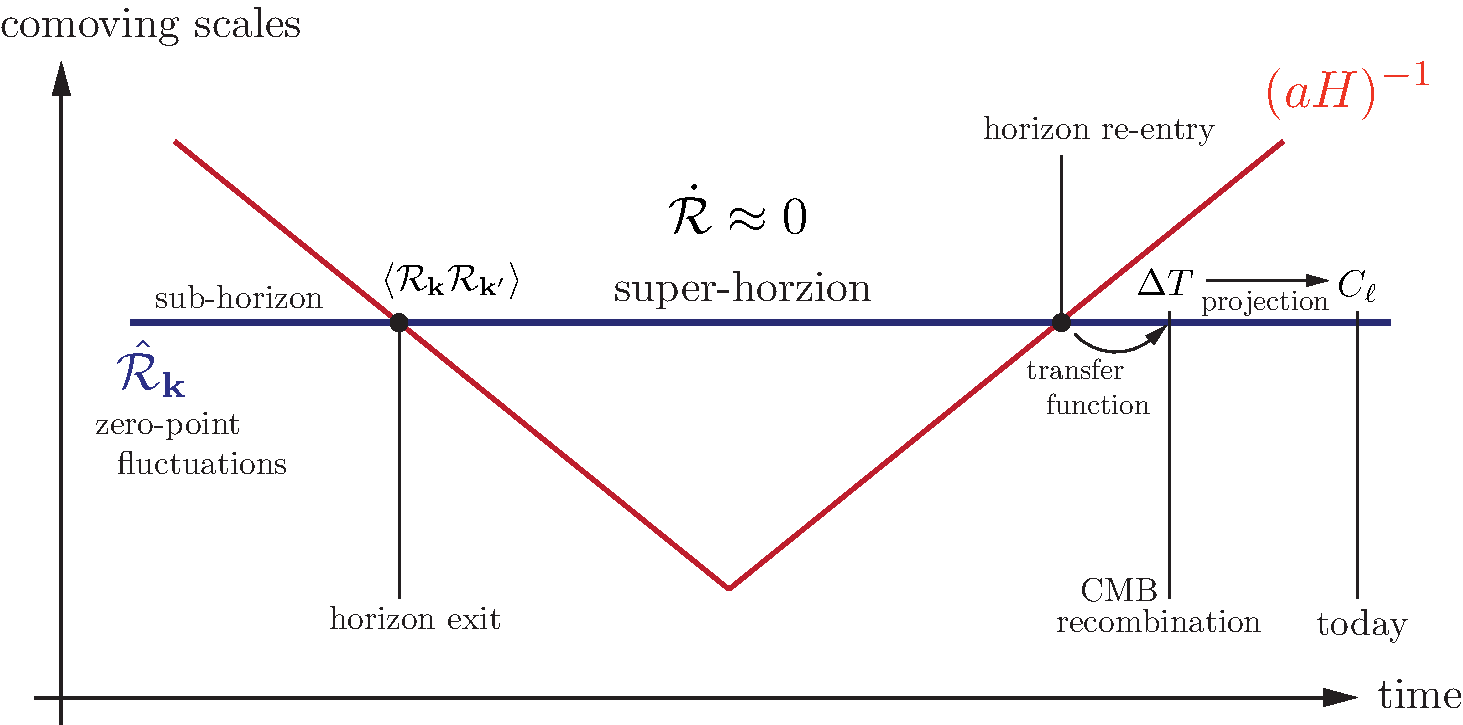
\includegraphics[width=0.75\textwidth]{./summary}
   \caption{\small インフレーション宇宙における摂動の生成と時間発展．揺らぎは地平線内のスケールで量子力学的に生成される（{\bf 第2講}参照）．共動スケール$k^{-1}$が一定に保たれる一方，インフレーション中の共動ハッブル半径$(aH)^{-1}$は縮小するため，摂動は地平線を退出し，後の時代に地平線へ再突入するまで凍結する．地平線再突入後，揺らぎはCMBの異方性とLSSの摂動へ発展する．宇宙論的観測を，インフレーションが刻んだ原始摂動に関係付けるには，この時間発展を考慮しなければならない（{\bf 第3講}参照）．}
    \label{fig:scales3}
\end{figure}

曲率摂動$\R$と重力波の振幅$h$は，モードが地平線を退出すると，$k=a(\tau_\star) H(\tau_\star)$，いずれも一定値で凍結する．
そのため前講では，地平線退出時$\tau_\star$の原始摂動を計算した．
これを宇宙論的観測量（CMB温度や銀河の密度など）に結び付けるには，次が必要である．
\begin{enumerate}
\item[i)] $\R$（または$h$）を，実験で実際に測定される量${\cal Q}$に関係付ける．
\item[ii)] 地平線へ再突入した後の$\R$（および${\cal Q}$）の時間発展を考慮する．
\end{enumerate}
模式的には，次のように書ける．
\beq
\fbox{$\displaystyle
{\cal Q}_{\bf k}(\tau) = T_{\cal Q}(k, \tau,\tau_\star) \, \R_{\bf k}(\tau_\star) $}\, ,
\eeq
ここで，$T_{\cal Q}$は，時刻$\tau_\star$での$\R$の揺らぎと，それより後のある時刻$\tau$での${\cal Q}$の揺らぎを結ぶ{\it 伝達関数}である．
表記からわかるように，伝達関数はスケールに依存しうる．
量${\cal Q}$は，ウィルキンソン・マイクロ波異方性探査機（WMAP）のようなCMB衛星が測定する温度揺らぎであっても，スローン・デジタル・スカイサーベイ（SDSS）のような銀河サーベイから推定する銀河密度であってもよい．


\vskip 6pt
\noindent
{\it CMB異方性}

\S\ref{sec:CMB}の主な結果は，インフレーションの入力スペクトル$P(k) \equiv \{ P_\R(k), P_h(k) \}$と，CMB温度揺らぎおよび偏光の角度パワースペクトルとの次の関係である．
\beq
\label{equ:CXY}
\fbox{$\displaystyle
C_\ell^{XY} = \frac{2}{\pi} \int k^2 \d k \underbrace{P(k)}_{\text{インフレーション}}\,  \underbrace{\Delta_{X \ell}(k) \Delta_{Y \ell}(k)}_{\text{異方性}} $}\, ,
\eeq
ここで，
\beq
\label{equ:source}
\Delta_{X \ell}(k) = \int_0^{\tau_0} \d \tau\, \underbrace{S_X(k, \tau)}_{\text{源}}\, \underbrace{P_{X\ell}(k[\tau_0-\tau])}_{\text{投影}}\, .
\eeq
添字$X,Y$は，温度$T$および偏光モード$E$と$B$を表す（\S\ref{sec:CMB}参照）．
積分(\ref{equ:CXY})は，インフレーションが予言する非一様性$P(k)$を，CMBで観測される異方性$C_\ell^{XY}$に結び付ける．異なる$X$および$Y$モード間の相関は，伝達関数$\Delta_{X\ell}(k)$と$\Delta_{Y\ell}(k)$によって関係付けられる．
伝達関数は，視線方向の積分(\ref{equ:source})として書ける．その被積分関数は，物理的な源の項$S_X(k, \tau)$と幾何学的な投影因子$P_{X\ell}(k[\tau_0-\tau])$（ベッセル関数の組合せ）に因数分解される．
源の項と投影因子の導出は本講の範囲を超えるが，Dodelsonの教科書\cite{Dodelson}にある．これらの結果の直観的な説明は，Wayne Huのウェブサイト\cite{WayneHu}にあるアニメーションで見られる．

本講での関心は，原始パワースペクトル$P_\R(k)$と$P_h(k)$に対する実験的制限にある．
原始スペクトルを測るには，適切な伝達関数と投影効果を考慮して，観測されたCMB異方性$C_{\ell}^{XY}$を{\it デコンボリューション}する必要がある．すなわち，背景宇宙論が与えられれば，式(\ref{equ:CXY})の時間発展と投影の効果を計算し，インフレーションの初期条件$P(k)$を取り出せる．このデコンボリューションの手続きによって，CMBは初期宇宙を探る魅力的な手段となる．

\vskip 6pt
\noindent
{\it 大規模構造}

物質分布の揺らぎ（例えば天球上の銀河分布によって測定される）を調べるため，密度コントラスト$\delta \equiv \delta \rho/ \bar \rho$を定義する．
銀河密度の揺らぎ$\delta_g$と暗黒物質密度の揺らぎ$\delta$は区別する．通常の仮定は，銀河が，その背後にある暗黒物質分布の（バイアスをもつ）トレーサーであるというもので，$\delta_g = b\, \delta$と書く．
{\it バイアス}パラメータ$b$を独立に決める方法があれば，銀河密度コントラスト$\delta_g$の観測から，背後の暗黒物質分布$\delta$を推定できる．
後期の暗黒物質密度揺らぎのパワースペクトルは，曲率揺らぎの原始スペクトルと次のように関係する．
\beq
\fbox{$\displaystyle
P_\delta(k, \tau) = \frac{4}{25} \left( \frac{k}{aH}\right)^4 T_\delta^2(k, \tau) P_\R(k)$}\, .
\eeq
伝達関数からくくり出した数値係数と$k$に関するスケーリングは，慣習によるものである．
伝達関数$T_\delta$は，物質優勢期の揺らぎの成長$\delta \sim a$と，放射優勢期の成長$\delta \sim \ln a$の違いを反映している．
通常，これは{\sf CMBFAST}~\cite{CMBFAST}や{\sf CAMB}~\cite{CAMB}などのコードを用いて数値的に計算する必要があるが，\S\ref{sec:T}では$T_\delta$の便利な近似関数を紹介する．
ここでも，背景宇宙論を固定すれば伝達関数は既知とみなせるので，物質パワースペクトルの観測は，初期宇宙に由来する初期揺らぎを探る手段になる．
%bias: relation between dark matter and galaxies; major uncertainty


\sectionlink{{\sl 復習}：宇宙マイクロ波背景放射}
\label{sec:CMB}


CMB揺らぎの物理と統計的解釈を，ごく簡単に復習する．
さらに詳しい説明は，Dodelsonの教科書\cite{Dodelson}や，{\sl TASI 2009}でのPierpaoli教授の講義にある．


\subsectionlink{温度異方性}

\subsubsection{球面調和関数展開}


 
\begin{figure}[h!]
    \centering
        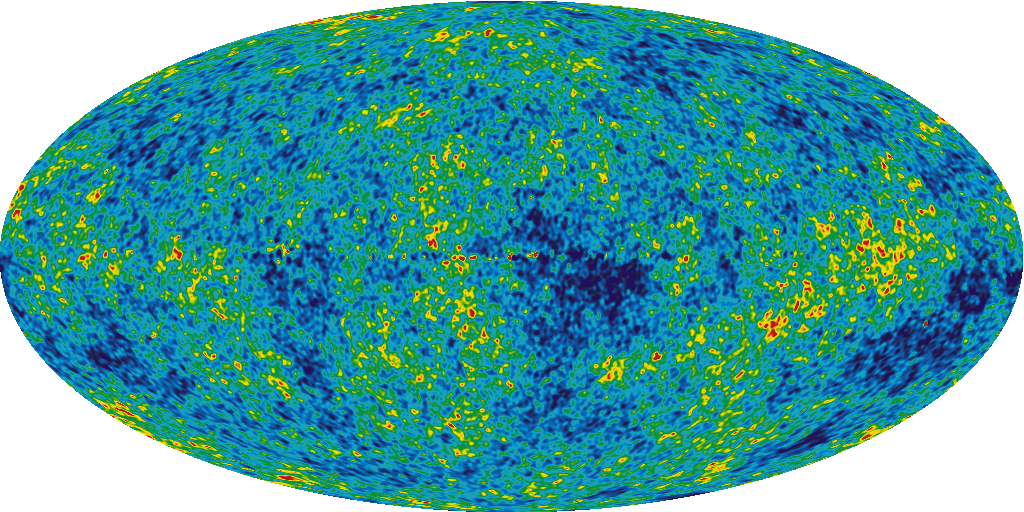
\includegraphics[width=0.7\textwidth]{cmb.png}
    \caption{\small CMBの温度揺らぎ．青い点は，CMB温度が平均値$T_0=2.7$ Kより$\sim 10^{-5}$低い天球上の方向を表す．これは，初期宇宙の高密度領域の重力ポテンシャルを登って脱出する際に，光子がエネルギーを失うことに対応する．黄色と赤は高温（低密度）の領域を表す．これらの揺らぎの統計的性質は，宇宙の背景の時間発展と初期条件の両方について重要な情報を含む．} % (see Figures \ref{fig:WMAP2} and \ref{fig:CMBparam}).}
    \label{fig:WMAP}
\end{figure} 

図\ref{fig:WMAP}は，背景温度$T_0 = 2.7$ Kに対して測定されたCMB温度揺らぎ$\Delta T(\hat n)$の地図を示す．
ここで，単位ベクトル$\hat n$は天球上の方向を表す．
この地図の球面調和関数展開は，
\beq
\label{equ:Tharm}
\Theta(\hat n) \equiv\frac{\Delta T(\hat n)}{T_0}= \sum_{\ell m} a_{\ell m} Y_{\ell m}(\hat n)\, ,
\eeq
ここで，
\beq
a_{\ell m} = \int \d \Omega\, Y^*_{\ell m}(\hat n) \Theta(\hat n)\, .
\eeq
ここで，$Y_{\ell m}(\hat n)$は2次元球面上の標準的な球面調和関数であり，$\ell=0$，$\ell=1$，$\ell=2$はそれぞれ単極子，双極子，四重極子に対応する．
磁気量子数は$m= - \ell, \dots , + \ell$を満たす．
多重極モーメント$a_{\ell m}$を組み合わせると，回転不変な角度パワースペクトルが得られる．% is defined as
\beq
\label{equ:Cl}
C_\ell^{TT} = \frac{1}{2\ell+1} \sum_m  \langle a^*_{\ell m} a_{\ell m} \rangle \, , \qquad \text{または} \qquad  \langle a^*_{\ell m} a_{\ell' m'} \rangle  = C_\ell^{TT} \delta_{\ell \ell'} \delta_{m m'}\, .
\eeq
角度パワースペクトルは，CMBの統計解析における重要な道具である．CMB地図の数百万画素に含まれる宇宙論的情報を，はるかにコンパクトなデータ表現で記述する．図\ref{fig:WMAP2}は，CMB角度パワースペクトルの最新の測定を示す．同図には，CMBスペクトルの理論予言をデータに当てはめた結果も示している．
理論曲線は，背景宇宙論のパラメータと初期揺らぎのスペクトルの両方に依存する．したがって，CMBでその両方を探ることができる．


\begin{figure}[h!]
    \centering
        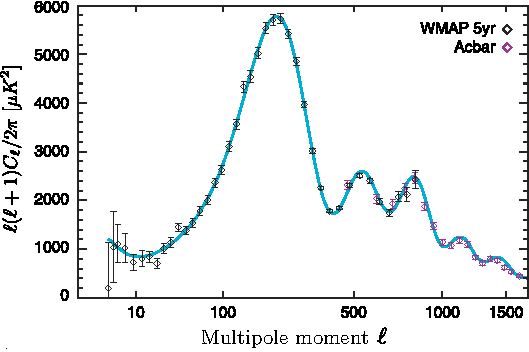
\includegraphics[width=0.65\textwidth]{WMAP_ACBAR}
    \caption{\small CMB温度揺らぎの角度パワースペクトル．} % (see Figures \ref{fig:WMAP2} and \ref{fig:CMBparam}).}
    \label{fig:WMAP2}
\end{figure} 


CMB温度揺らぎは，{\it スカラー}モード$\R$によって支配される（少なくとも，現在考慮されているテンソル・スカラー比$r <0.3$の範囲では）．
$\R$と$\Delta T$を結ぶ線形の時間発展は，伝達関数$\Delta_{T \ell}(k)$を通じ，次の$k$空間積分で与えられる\cite{Dodelson}．
\beq
\label{equ:alm} 
\fbox{$\displaystyle
a_{\ell m} = 4\pi (-i)^\ell \int \frac{\d^3 k}{(2\pi)^3} \, \Delta_{T \ell}(k)\, \R_{\bf k} \, Y_{\ell m}(\hat {\bf k}) $}\, .
\eeq
式(\ref{equ:alm})を(\ref{equ:Cl})に代入し，恒等式
\beq
\sum_{m=-\ell}^\ell Y_{\ell m}(\hat {\bf k}) Y_{\ell m}(\hat {\bf k}') = \frac{2\ell+1}{4\pi} P_\ell(\hat {\bf k} \cdot \hat {\bf k}')\, ,
\eeq
を用いると，
\beq
\label{equ:Cl2}
C_\ell^{TT} = \frac{2}{\pi} \int k^2 \d k \underbrace{P_\R(k) }_{\text{インフレーション}} \underbrace{\Delta_{T \ell}(k) \Delta_{T \ell}(k)}_{\text{異方性}} \, .
\eeq
伝達関数$\Delta_{T\ell}(k)$は一般に，{\sf CMBFAST}~\cite{CMBFAST}や{\sf CAMB}~\cite{CAMB}などのボルツマン計算コードを用いて数値計算する必要がある．これらは背景宇宙論のパラメータに依存する．背景宇宙論を固定すると，パワースペクトル$C_{\ell}^{TT}$の形は，原始パワースペクトル$P_\R(k)$で記述される初期条件についての情報を含む．\footnote{実際には，CMBデータに対して，背景宇宙論と揺らぎのスペクトルを同時に当てはめる．}もちろん，観測から$P_\R(k)$，したがってインフレーションについて学ぶことが，本講の主な目的である．
%where
%\beq
%\Delta_{T \ell}(k) = \int_0^{\tau_0} \d \tau\, \underbrace{S_T(k, \tau)}_{\rm Sources}\, \underbrace{P_{T\ell}(k[\tau_0-\tau])}_{\rm Projection}
%\eeq


\subsubsection{大きなスケール}

大きなスケールのモードは，再結合時にはまだ地平線の外側にあった．
したがって，大スケールのCMBスペクトルは地平線内の時間発展の影響を受けておらず，再結合時の原始スペクトルを現在のわれわれの位置へ幾何学的に投影したものにすぎない．
この{\it ザックス＝ヴォルフェ領域}では，伝達関数$\Delta_{T\ell}(k)$は単なるベッセル関数である\cite{Dodelson}．
\beq
\Delta_{T \ell}(k) = \frac{1}{3} j_\ell(k[\tau_0-\tau_{\rm rec}])\, .
\eeq
したがって，大きなスケール（小さい$\ell$）での角度パワースペクトルは，
\beq
\label{equ:Cl3}
C_\ell^{TT} = \frac{2}{9 \pi} \int k^2 \d k \, P_\R(k) \, j_\ell^2(k[\tau_0-\tau_{\rm rec}]) \, .
\eeq
ベッセル投影関数は$k[\tau_0-\tau_{\rm rec}] \approx \ell$にピークをもち，実質的に$k$と$\ell$を対応付ける$\delta$関数のように作用する．
波数$k\approx \ell/(\tau_0-\tau_{\rm rec})$のモードが式(\ref{equ:Cl3})の積分を支配することから，次のように書ける．
\beq
C_\ell^{TT} \propto \left. k^3 P_\R(k) \right|_{k\approx \ell/(\tau_0-\tau_{\rm rec})} \underbrace{\int \d \ln x \ j^2_\ell(x)}_{\propto\, \ell(\ell+1)}\, .
\eeq
したがって，
\beq
\ell(\ell+1) C_\ell^{TT} \propto \left. \Delta_{\rm s}^2(k) \right|_{k\approx \ell/(\tau_0-\tau_{\rm rec})} \propto \ell^{\, n_{\rm s}-1}\, .
\eeq
入力スペクトルがスケール不変$n_{\rm s} =1$の場合，次の量は，
\beq
{\cal C}_\ell \equiv \frac{\ell(\ell+1)}{2\pi} C_\ell^{TT}
\eeq
$\ell$に依存しない（ただし，暗黒エネルギー優勢の宇宙で重力ポテンシャルが後期に時間発展することで生じる，積分ザックス＝ヴォルフェ効果による非常に小さい$\ell$での増加を除く）．
このため，CMBパワースペクトルは$C_\ell^{TT}$の代わりに${\cal C}_\ell$で描かれることが多い．


\subsubsection{非ガウス性}

ここまで，地平線内の時間発展と幾何学的投影効果を考慮すれば，CMB揺らぎの角度パワースペクトルが実質的に原始パワースペクトル$P_\R(k)$の尺度となることを示した．
\beq
\langle a^*_{\ell m} a_{\ell' m'} \rangle = C_\ell^{TT} \delta_{\ell \ell'} \delta_{m m'} \quad \Leftrightarrow \quad 
\langle \R_{{\bf k}} \R_{{\bf k}'} \rangle = (2\pi)^3 P_\R(k)\, \delta({\bf k} + {\bf k}')\, .
\eeq
原始揺らぎがガウス的なら，$P_\R(k)$がすべての情報を含む．
実際，単一場スローロール・インフレーションは，$\R$が非常に高い精度でガウス的になると予言する\cite{malda}．
しかし，{\bf 第4講}で説明するように，たとえわずかな非ガウス性であっても，最も単純な単一場スローロール模型を超える必要があることを意味するため，インフレーションの作用について重要な情報を与える．

非ガウス性の主な尺度は，{\it 3点関数}，またはそれと等価な{\it バイスペクトル}である．
\beq
 \langle \R_{{\bf k}_1} \R_{{\bf k}_2} \R_{{\bf k}_3}\rangle = (2\pi)^3 B_\R(k_1,k_2,k_3)\, \delta({\bf k}_1 + {\bf k}_2+{\bf k}_3)\, .
\eeq
CMBでは，ゼロでないバイスペクトル$B_\R(k_1, k_2, k_3)$が，角度バイスペクトルに痕跡を残す．
\beq
\label{equ:Bl0}
B^{\ell_1 \ell_2 \ell_3}_{m_1 m_2 m_3} = \langle a_{\ell_1 m_1} a_{\ell_2 m_2} a_{\ell_3 m_3}\rangle \, .\eeq
式(\ref{equ:alm})を(\ref{equ:Bl0})へ代入すると，原始バイスペクトルを，観測されるCMBバイスペクトルに結び付けられる\cite{NGreview}．\footnote{非線形の時間発展は，さらに非ガウス性を生じさせることがある（{\bf 第4講}参照）．}

原始バイスペクトル$B_\R(k_1,k_2,k_3)$は，運動量保存だけを制約とする三つの運動量の関数であることに注意しよう（すなわち，三つのベクトル${\bf k}_i$は閉じた三角形をなす）．
このため，非ガウス性への観測的制限を得るのは難しい（考慮すべき非ガウス性の形が多数ある）．一方，検出されれば，非ガウス性には初期宇宙の物理について多くの情報が含まれるということでもある．

原始非ガウス性の簡単な模型は{\it 局所型非ガウス性}であり，曲率摂動をそのガウス成分$\R_g$の周りでテイラー展開して定義される．
\beq
\label{equ:localx}
\R({\bf x}) = \R_g({\bf x}) + \frac{3}{5} f_{\rm NL}^\R \star \R_g^2({\bf x})\, .
\eeq
これは実空間で局所的であり，パラメータ$f_{\rm NL}^\R$が非ガウス性の大きさを特徴付ける．
式(\ref{equ:localx})から，バイスペクトルについて次の簡単な形が得られることを，読者は確かめてみてほしい．
\beq
B_\R(k_1,k_2,k_3) = \frac{6}{5} f_{\rm NL}^\R \Bigl[ P_\R(k_1) P_\R(k_2) + P_\R(k_2) P_\R(k_3) + P_\R(k_3) P_\R(k_1)\Bigr]\, .
\eeq
したがって，現在の非ガウス性への観測的制限は，パラメータ$f_{\rm NL}^\R$への制限として述べられることが多い（\S\ref{sec:evidence}参照）．

\subsectionlink{偏光}

CMB偏光は，初期宇宙を支配する物理を探る最も重要な手段の一つになると考えられる．
CMBの温度異方性に加え，CMBはトムソン散乱によって偏光すると期待される\cite{Dodelson}．これから説明するように，この偏光には原始揺らぎ，したがってインフレーションについての重要な情報が含まれる\cite{WhitePaper}．

\begin{figure}[htbp!]
    \centering
        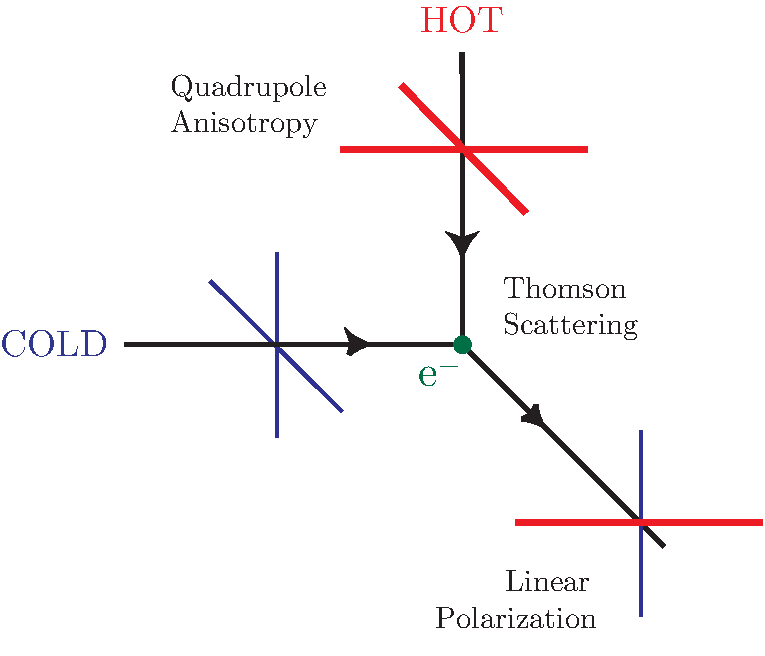
\includegraphics[width=0.55\textwidth]{PolarizationV3}
   \caption{四重極異方性をもつ放射のトムソン散乱によって，直線偏光が生成される．ここで，赤い（太い）線は高温の放射を，青い（細い）線は低温の放射を表す．}
    \label{fig:pol}
\end{figure}

\subsubsection{トムソン散乱による偏光}

%Thomson scattering between electrons and photons produces a simple relationship between temperature anisotropy and polarization.
光子と自由電子の散乱によって偏光がどのように生成されるかを見てみよう．
入射放射の分布が（電子の静止系で）等方的なら，直交する偏光方向が互いに打ち消し合うため，出てくる放射は無偏光のままである．
正味の直線偏光が生じるのは，入射放射場に四重極成分がある場合だけである（図\ref{fig:pol}参照）．
このような四重極モーメントは，再結合の直前に光子が電子や陽子から脱結合するときに生成される．温度異方性は原始密度揺らぎによって作られるので，偏光の一成分は温度異方性と相関するはずである．


\subsubsection{放射場の特徴付け}

%We digress briefly to give details of the mathematical characterization of CMB temperature and polarization anisotropies.
CMB偏光異方性の数学的な特徴付けは，温度揺らぎの記述より少し複雑である．偏光はスカラー場ではないため，通常の球面調和関数による展開が適用できないからである．

異方性の場は，$2\times 2$の強度テンソル$I_{ij}(\hat n)$で定義される．ここで，これまでと同様に$\hat n$は天球上の方向を表す．$I_{ij}$の成分は，$\hat n$に垂直な二つの直交基底ベクトル$\hat{\bf e}_1$と$\hat {\bf e}_2$に対して定義される．
直線偏光はストークスパラメータ$Q = \frac{1}{4}(I_{11}-I_{22})$と$U=\frac{1}{2} I_{12}$で記述され，温度異方性は$T = \frac{1}{4} (I_{11}+I_{22})$である．
偏光の大きさと角度は，それぞれ$P =\sqrt{Q^2 +U^2}$と$\alpha = \frac{1}{2} \tan^{-1}(U/Q)$である．
量$T$は$\hat n$に垂直な平面内での回転に不変なので，スカラー（スピン0）の球面調和関数(\ref{equ:Tharm})で展開できる．
%\beq
%T(\hat n) = \sum_{\ell, m}  a_{\ell m}^T\ Y_{\ell m}(\hat n)\, .
%\eeq
一方，量$Q$と$U$は，角度$\psi$の回転の下でスピン2の場として変換し，$(Q \pm iU)(\hat n) \to e^{\mp 2 i \psi} (Q \pm i U)(\hat n)$となる．したがって，$Q \pm i U$の調和解析には，テンソル（スピン2）の球面調和関数による球面上の展開が必要である\cite{Kamionkowski:1996ks, Zaldarriaga:1996xe, NewmanPenrose}．
\beq
(Q \pm iU)(\hat n) = \sum_{\ell, m}  a_{\pm 2,\ell m} \, {}_{\pm 2}Y_{\ell m}(\hat n)\, .
\eeq
これらのテンソル球面調和関数${}_{\pm 2}Y_{\ell m}$の数学的性質を説明すると，本講の主題から外れすぎるので，古典的な論文\cite{Kamionkowski:1996ks, Zaldarriaga:1996xe}やDodelsonの教科書\cite{Dodelson}を参照してほしい．

\subsubsection{$E$モードと$B$モード}
モーメント$a_{\pm2,\ell m}$の代わりに，次の線形結合を導入すると便利である．%\cite{NewmanPenrose}
\beq
a_{E, \ell m} \equiv -\frac{1}{2} \left(a_{2, \ell m} + a_{-2, \ell m}\right)\, , \qquad
a_{B, \ell m} \equiv - \frac{1}{2i} \left(a_{2, \ell m} - a_{-2, \ell m}\right)\, .
\eeq
すると，スピン2の量$Q$と$U$の代わりに，二つのスカラー（スピン0）の場を定義できる．
\beq
E(\hat n) = \sum_{\ell, m} a_{E, \ell m}\, Y_{\ell m}(\hat n)\, , \qquad B (\hat n)=\sum_{\ell, m} a_{B, \ell m}\, Y_{\ell m}(\hat n)\, .
\eeq

\begin{figure}[htbp!]
    \centering
        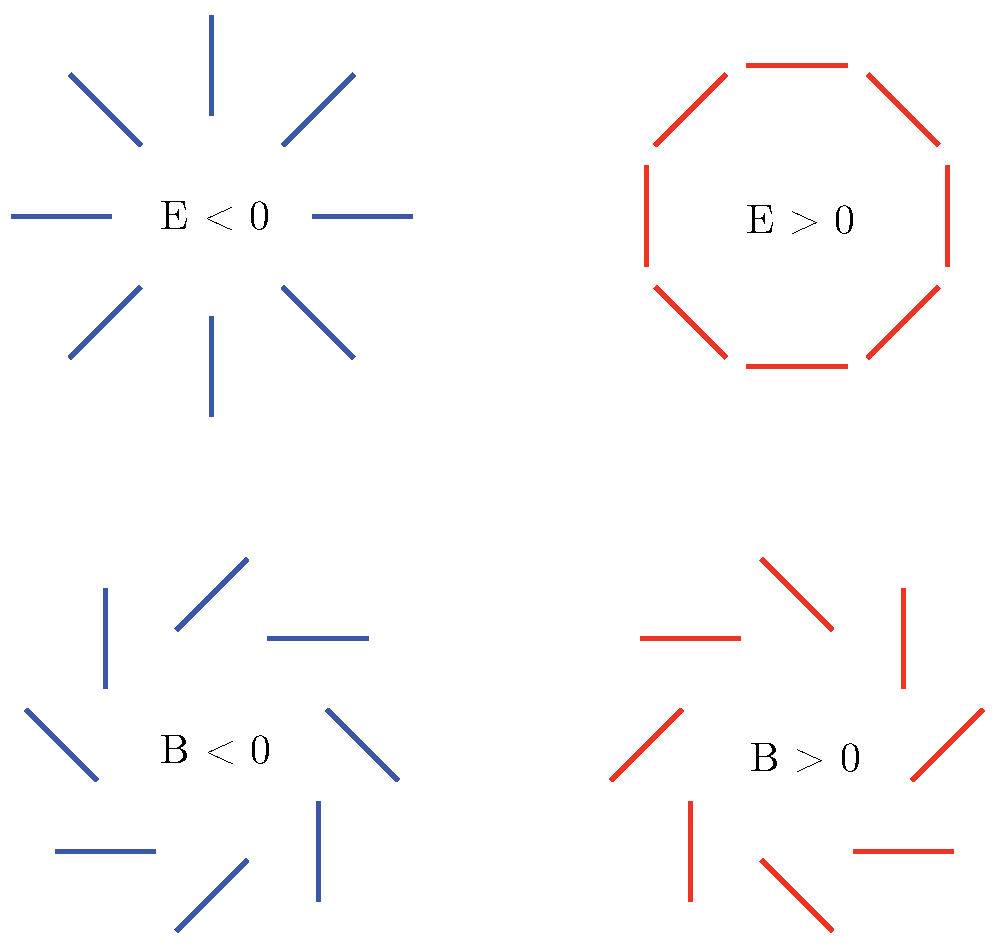
\includegraphics[width=.45\textwidth]{EBmode}
   \caption{偏光の$E$モードと$B$モードのパターンの例．中心を通る直線に関して反転すると，$E$モードのパターンは変わらない一方，正と負の$B$モードのパターンは入れ替わることに注意しよう．}
    \label{fig:EBmode}
\end{figure}

スカラー量$E$と$B$は，直線偏光の場を完全に指定する．
$E$モード偏光は，天球上の低温点の周りで偏光ベクトルが放射状となり，高温点の周りでは接線方向となる，{\it 回転のない}モードとしても特徴付けられる．
一方，$B$モード偏光は{\it 発散がない}が{\it 回転をもつ}．その偏光ベクトルは，天球上の各点の周りに渦度をもつ．\footnote{$E$と$B$という名称は明らかに，静電磁場でおなじみの性質$\nabla \times {\bf E} = 0$と$\nabla \cdot {\bf B} = 0$を反映している．}
図\ref{fig:EBmode}に，$E$モードと$B$モードのパターンの例を示す．
$E$と$B$はいずれも回転に不変だが，パリティ変換の下では異なる振る舞いをする．%$E$-polarization remains unchanged and $B$-polarization changes sign.
中心を通る直線に関して反転したとき，$E$モードのパターンは変わらないが，$B$モードのパターンは符号を変えることに注意しよう．

温度と偏光（$E$モードおよび$B$モード）の異方性の対称性は，4種類の相関を許す．すなわち，温度揺らぎ，$E$モード，$B$モードの自己相関で，それぞれ$TT$，$EE$，$BB$と表されるもの，および温度揺らぎと$E$モードとの相互相関$TE$である．それ以外の相関（$TB$と$EB$）は，対称性のためにすべて消える．
%\footnote{This assumes no parity-violating processes in the early universe.  Conversely, non-zero $TB$ and $EB$ correlations would be a distinctive signature  of such physics.}
  % All these statements apply to primary anisotropies
  %only; at the level of secondary anisotropies, non-zero $TB$ and $EB$-correlations are generated by weak lensing effects.}

角度パワースペクトルは，これまでと同様に定義する．
\beq
C_\ell^{XY} \equiv \frac{1}{2\ell + 1} \sum_m \langle a_{X,\ell m}^* a_{Y,\ell m} \rangle \, , \qquad X, Y = T, E, B\, .
\eeq
図\ref{fig:TE}には，$TE$相互相関の最新の測定\cite{WMAP5}を示す．$EE$スペクトルの測定も始まっているが，誤差はまだ大きい．これまでのところ，$BB$スペクトルについては上限しか得られておらず，検出には至っていない．

\begin{figure}[htbp!]
    \centering
        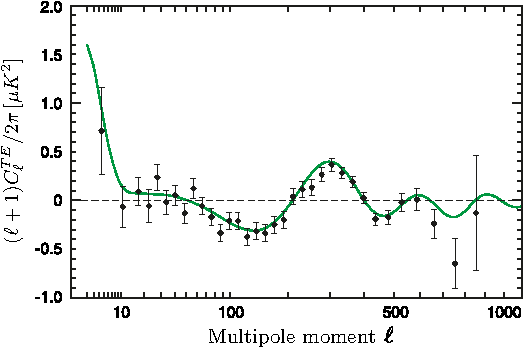
\includegraphics[width=.65\textwidth]{TEv2}
   \caption{温度異方性と$E$モード偏光異方性の相互相関のパワースペクトル\cite{WMAP5}．$\ell = 50-200$（角距離$5^\circ > \theta > 1^\circ$に対応）での反相関は，脱結合期の地平線より大きなスケールにおける断熱揺らぎの特徴的な徴候であり\cite{spergel/zaldarriaga:1997, Dodelson:2003ip}，インフレーションの枠組みの基本的な予言を裏付ける．}
    \label{fig:TE}
\end{figure}

CMB偏光の$E$/$B$分解の宇宙論的な重要性は，文献\cite{Kamionkowski:1996ks, Zaldarriaga:1996xe}の著者らによって認識された．彼らは次の注目すべき事実を証明した．
\begin{enumerate}
\item[i)] スカラー（密度）摂動は$E$モードだけを生成し，$B$モードを{\it 生成しない}．
\item[ii)] ベクトル（渦度）摂動は主として$B$モードを生成する．\footnote{しかし，ベクトルは宇宙の膨張とともに減衰するので，再結合時には劣勢だと考えられている．したがって，ここでは考慮しない．}
%, but note that cosmic strings can produce a $B$-mode signal via vector modes (see \S\ref{sec:defects}).}
\item[iii)] テンソル（重力波）摂動は$E$モードと$B$モードの両方を生成する．
\end{enumerate}
%Intuitively these results may be understood as follows:
%Thomson scattering produces an $E$-mode locally at the scattering event.
%For scalar perturbations the spatial pattern of the polarization field at the last-scattering surface is curl-free. Since free streaming (to linear order) projects a curl-free spatial pattern to a curl-free angular distribution, the observed signal from scalar perturbations remains curl-free and hence pure $E$-mode.
%For tensor modes the polarization is also $E$-mode at last scattering, but the spatial distribution has non-zero curl. Projection of the polarization pattern from the last-scattering surface to the point of observation today therefore produces $B$-mode polarization.

{\it スカラーは$B$モードを生成しない}が，{\it テンソルは生成する}という事実が，$B$モードの検出はテンソルモード，したがってインフレーションの決定的証拠であるという主張の根拠となる．
%The search for the primordial  $B$-mode signature of inflation is often considered the ``holy grail" of observational cosmology.
%We discuss the theoretical implications of the $B$-mode amplitude in Section~\ref{sec:Bmodes}.


\subsubsection{$E$モードとスカラー}

$E$モードのパワースペクトルと$TE$相互相関は，インフレーションの{\it スカラー}モードによって支配される．すなわち，
\bea
C_\ell^{EE} &\approx& (4\pi)^2 \int k^2 \d k \overbrace{P_\R(k) }^{\text{インフレーション}} \Delta_{E \ell}^2(k) \, ,\\
%\underbrace{\Delta_{B \ell}(k) \Delta_{B \ell}(k)}_{\rm Anisotropies} 
C_\ell^{TE} &\approx& (4\pi)^2 \int k^2 \d k \underbrace{P_\R(k) }_{\text{インフレーション}} \Delta_{T\ell}(k) \Delta_{E \ell}(k)\, .
%\underbrace{\Delta_{B \ell}(k) \Delta_{B \ell}(k)}_{\rm Anisotropies} 
\eea
$C_\ell^{TT}$と同様に，スペクトル$C_\ell^{EE}$と$C_\ell^{TE}$は$P_\R(k)$についての情報を与える．
しかし，それぞれの場合で原始スペクトルは異なる伝達関数と畳み込まれるため（偏光は自由電子による散乱だけで生成される），これらの信号は有用な相補性をもつ．

\subsubsection{$B$モードとテンソル}

$B$モードは{\it テンソル}モードだけによって生成される．すなわち，
\beq
C_\ell^{BB} = (4\pi)^2 \int k^2 \d k \underbrace{P_h(k) }_{\text{インフレーション}} \Delta_{B \ell}^2(k)\, .
%\underbrace{\Delta_{B \ell}(k) \Delta_{B \ell}(k)}_{\rm Anisotropies} 
\eeq
%where
%\beq
%\Delta_{B \ell}(k) = \int_0^{\tau_0} \d \tau\, \underbrace{S_B(k, \tau)}_{\rm Sources}\, \underbrace{P_{B\ell}(k[\tau_0-\tau])}_{\rm Projection}
%\eeq
したがって，$C_\ell^{BB}$の測定は，原始テンソル揺らぎの情報を得る独自の機会となる．

\begin{figure}[h!]
    \centering
        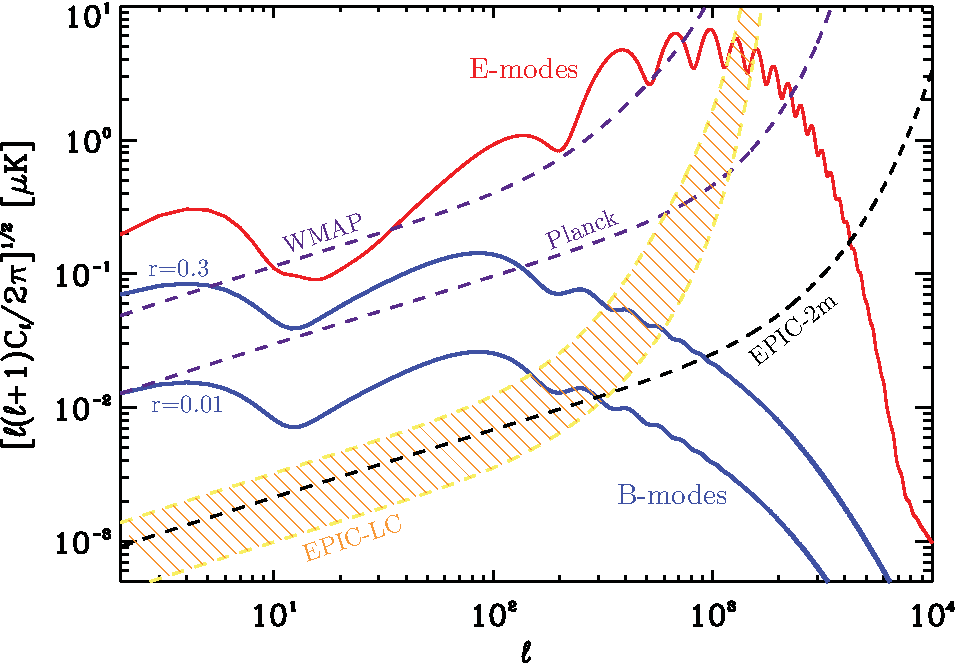
\includegraphics[width=0.65\textwidth]{EPIC}
    \caption{現在の上限に等しいテンソル・スカラー比$r=0.3$，および$r=0.01$に対する$E$モードと$B$モードのパワースペクトル．{\sl WMAP}，{\sl Planck}，および将来のCMB衛星（{\sl CMBPol}）の二つの異なる設計案（EPIC-LCとEPIC-2m）の実験感度も示している\cite{EPIC}．}
    %({\small Figure adapted from Bock {\it et al.}~\cite{EPIC}.})}
    \label{fig:spectra}
\end{figure}


\sectionlink{{\sl 復習}：大規模構造}

\begin{figure}[h!]
    \centering
        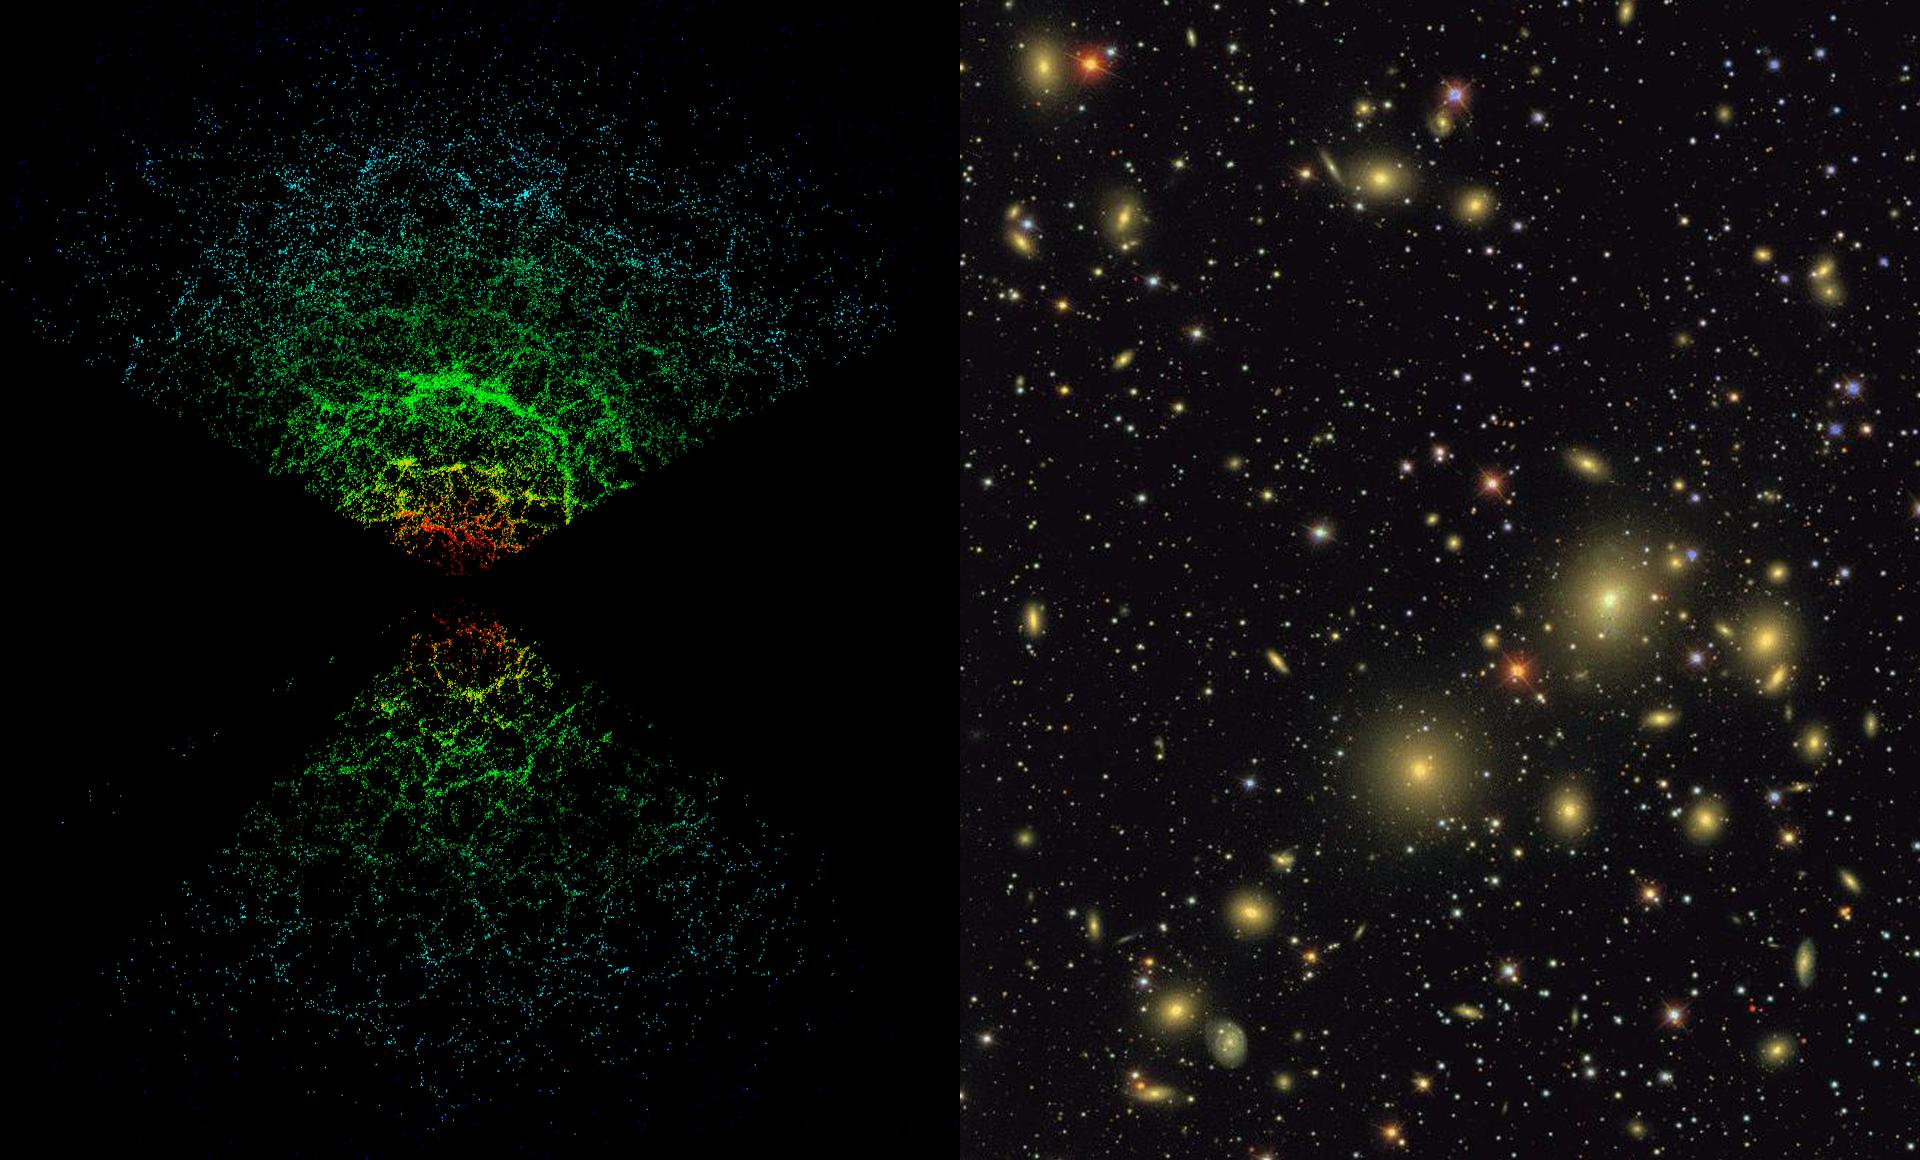
\includegraphics[width=.9\textwidth]{galaxies.jpg}
    \caption{\small 銀河の分布．スローン・デジタル・スカイサーベイ（SDSS）は，約100万個の銀河の位置と距離（赤方偏移）を測定した．
    まず右上のような2次元画像で同定した銀河について，距離を測定して3次元地図を作る．左の画像は，そのような3次元地図の一断面を示す．測定された銀河分布の統計的性質は，後期宇宙の構造と進化について重要な情報を明らかにする．}
    \label{fig:SDSS}
\end{figure}

銀河（または暗黒物質）のパワースペクトルは，原始曲率揺らぎのスペクトルの尺度となる．
\beq
P_\delta(k, z) \quad \Rightarrow \quad P_\R(k)\, ,
\eeq
ただし，地平線内の時間発展の効果を考慮する必要がある．
これは，暗黒物質の伝達関数によって行う．

\subsectionlink{暗黒物質の伝達関数}
\label{sec:T}


密度揺らぎは，圧力と重力の競合の下で時間発展する．
放射優勢期には，強い放射圧が揺らぎの急速な成長を妨げるため，密度コントラストは対数的にしか成長せず，$\delta \sim \ln a$となる．
物質優勢期には，背景の圧力が無視でき，重力収縮がより効果的に働くため，$\delta \sim a$となる．

地平線突入から物質優勢期までの間に摂動が有意には成長しないという簡単化の仮定の下では，次の近似的な伝達関数を導ける．
\beq
\label{equ:Tapprox}
T_\delta(k) \approx \left\{ \begin{array}{l l} 1 & k < k_{\rm eq} \\ (k_{\rm eq}/k)^2 & k > k_{\rm eq} \end{array} \right. \, .
\eeq
式(\ref{equ:Tapprox})は，スペクトルの定性的な形（すなわち$k \approx k_{\rm eq}$でのスペクトルの折れ曲がり）を直観的に理解するには有用だが，ほとんどの応用に対して精度が足りない．
物質の伝達関数に対する有名な近似関数は，Bardeenら（BBKS）\cite{BBKS}によって与えられた．
\beq
T_\delta(q) = \frac{\ln(1+2.34 q)}{2.34 q} \left[ 1+ 3.89 q +(1.61 q)^2 +(5.46 q)^3 + (6.71 q)^4\right]^{-1/4}\, ,
\eeq
ここで，$q=k/\Gamma h\, {\rm Mpc}^{-1}$であり，形状パラメータを次のように定義した．
\beq
\Gamma \equiv \Omega h \exp (-\Omega_b - \sqrt{2h} \Omega_b/\Omega)\, .
\eeq
より正確な伝達関数は，EisensteinとHu\cite{EisensteinHu}にある．
最後に，厳密な伝達関数は{\sf CMBFAST}~\cite{CMBFAST}または{\sf CAMB}~\cite{CAMB}で数値計算できる．

われわれの目的にとって重要なのは，（背景宇宙論のパラメータが与えられれば）暗黒物質の伝達関数を計算でき，それを用いて暗黒物質パワースペクトル$P_\delta(k,z)$をインフレーションのスペクトル$P_{\cal R}(k)$に関係付けられる，という点だけである．

\subsectionlink{銀河バイアス}

残念ながら，重力レンズを除けば暗黒物質を直接観測できない．
（例えばスローン・デジタル・スカイサーベイ（SDSS）のような銀河サーベイで）観測するのは，光を放つ物質，すなわちバリオン物質である．
大きなスケールでは，銀河分布と暗黒物質を結び付ける次の現象論的な仮定が有用であることがわかっている．
\beq
\delta_g = b\, \delta\, ,
\eeq
あるいは，
\beq
P_{\delta_g} = b^2 P_\delta\, .
\eeq
ここで，$b$は（線形）バイアスパラメータと呼ばれる．これは，十分に理解されていない銀河形成の物理を記述するパラメータとみなせる．
バイアスパラメータ$b$は，銀河のバイスペクトル$B_{\delta_g}$を測定して求められる．

こうした複雑さを別にすれば，銀河パワースペクトル$P_{\delta_g}(k)$は，インフレーションのスカラー揺らぎ$P_\R(k)$を探る追加の手段となる．より小さなスケールを調べるため，CMB揺らぎの観測と相補的である．

%\newpage
\sectionlink{インフレーションを支持する現在の証拠}
\label{sec:evidence}

インフレーションは仮説である．
インフレーションが初期宇宙の物理的実在を記述しているという確信を高めるため，その予言を宇宙論的観測と比較する．
本節では，インフレーションを支持する現在の観測的証拠を説明し，次節で将来の検証を論じる．


\subsectionlink{平坦性}

宇宙は，バリオン，暗黒物質，光子，ニュートリノ，暗黒エネルギーで満たされている．
\beq
\Omega_{\rm tot} = \Omega_b + \Omega_{\rm cdm} + \Omega_\gamma + \Omega_\nu + \Omega_\Lambda\, .
\eeq
$\Omega_{\rm tot}$の値は宇宙の空間幾何を決め，$\Omega_{\rm tot}=1$は平坦な宇宙，$\Omega_{\rm tot} < 1$は負の曲率をもつ宇宙，$\Omega_{\rm tot} > 1$は正の曲率をもつ宇宙に対応する．
インフレーションの予言は，
\beq
\Omega_{\rm tot} = 1 \pm 10^{-5}\, ,
\eeq
一方，データは次を示す\cite{WMAP5}．
\beq
\Omega_{\rm tot} = 1 \pm 0.02\, .
\eeq
この理論とデータの一致は見事だが，インフレーションは宇宙の平坦性を，ある意味「設計どおり」に実現しているとも言える．\footnote{ただし，グースが1980年にインフレーションを導入した時点では，宇宙の平坦性は非自明な予言であり，当時の観測と矛盾していたことは指摘しておく価値がある！}
したがって，インフレーションという考え方の追加の検証を探すべきである．


\subsectionlink{位相のコヒーレンスと地平線外の揺らぎ}

本講義で繰り返し強調してきたように，非一様な宇宙の観測によって，インフレーションの力学を詳しく検証できる．
この小節では，インフレーションが自然に説明する，観測の非自明な定性的特徴を論じ，次の小節で定量的な結果を示す．

%\vskip 6pt
以下は，Dodelsonが文献\cite{Dodelson:2003ip}で美しく説明した議論を単純化したものである．

\subsubsection{TTスペクトルのピーク}

インフレーションは，ほぼスケール不変な摂動スペクトルを生成する．
\beq
\langle \R_{\bf k} \R_{\bf k'} \rangle = (2\pi)^3 \delta ({\bf k} +{\bf k}') P_\R(k)\, ,
\eeq
ここで，$k^3 P_\R(k) \propto k^{n_{\rm s}-1}$であり，$n_{\rm s} \approx 1$である．
\begin{quote}
そうすると，パワースペクトルの形を観測で測定でき，それによってインフレーションの正しさを確信するのだと思うかもしれない．確かに，物質と放射の両方についてパワースペクトルを測定でき，観測が理論と一致するのも確かである．しかし，データを見て背筋が震えるのはそのためではない．インフレーション中に生成された摂動の真に驚くべき特徴は，むしろ，{\it すべてのフーリエモードが同じ位相をもつ}ことである\cite{Dodelson:2003ip}．
\end{quote}
物理的波長$\lambda$のフーリエモードを考えよう．インフレーション中に地平線の内側にある間，モードは$k = 2\pi/\lambda$で与えられる振動数で振動する．しかし，インフレーションが終わる前に，モードは地平線を退出する．すなわち，その物理的波長が，その時点のハッブル半径より長く引き伸ばされ，$\lambda > H^{-1}$となる．その後，振幅は一定に保たれる．ずっと後にモードが地平線へ再突入して初めて，因果的な物理過程が作用し，時間発展を起こせるようになる．
揺らぎの振幅は地平線の外側で一定だったので，地平線再突入時の$\dot \R$は非常に小さい．
一般には，各フーリエモードは正弦モードと余弦モードの線形結合でありうる．しかし，インフレーションの特別な点は，余弦モードだけを励起することである（地平線再突入時を$t \equiv 0$と定義する）．

地平線の内側に入ると，曲率摂動$\R$は密度揺らぎ$\delta$の源となり，密度揺らぎは重力と圧力の影響の下で時間発展する．
\beq
\ddot \delta - c_s^2 \nabla^2 \delta = F_g[\R]\, ,
\eeq
ここで，$c_s$は音速，$F_g$は重力の源の項である．
これにより密度場に振動が生じる．初期宇宙のプラズマでは，物質密度の揺らぎは放射の揺らぎと強く結合していた．したがって，CMB揺らぎは，再結合時の背後にある密度場の状態を直接写したスナップショットを与える．
再結合が瞬間的に起こると想像しよう（これはそれほど悪い近似ではない）．
波長の異なる揺らぎは，それぞれの振動の異なる位相で捉えられるだろう．
ある波長のモードは振幅が最大または最小の時点で捉えられ，別の波長のモードは振幅がゼロの時点で捉えられる．
ある波長をもつすべてのフーリエモードの位相が揃っていれば，それらはコヒーレントに干渉し，全フーリエモードのスペクトルは，最終散乱面に見えるCMBパワースペクトルに一連の山と谷を生む．
これはもちろん，図\ref{fig:WMAP}で見ているものである．しかし，初期揺らぎの理論がこれを説明するには，すべてのフーリエモードにコヒーレントな初期位相を生む機構が必要である．インフレーションはまさにそれを行う！
揺らぎは地平線を退出すると凍結するため，フーリエモードの位相は，関心のあるモードが地平線へ入るよりもずっと前に定まっていた．CMBパワースペクトルのピーク構造に感嘆するとき，実際に感嘆しているのは，原始揺らぎを生む機構が，すべてのフーリエモードの位相を揃える能力である．このコヒーレンスがなければ，CMBパワースペクトルは山も谷もない単なる白色雑音となる（実際，宇宙ひもや位相的欠陥が原始揺らぎの主な源として排除されるのは，まさにこの理由である）．

\begin{figure}[h!]
    \centering
        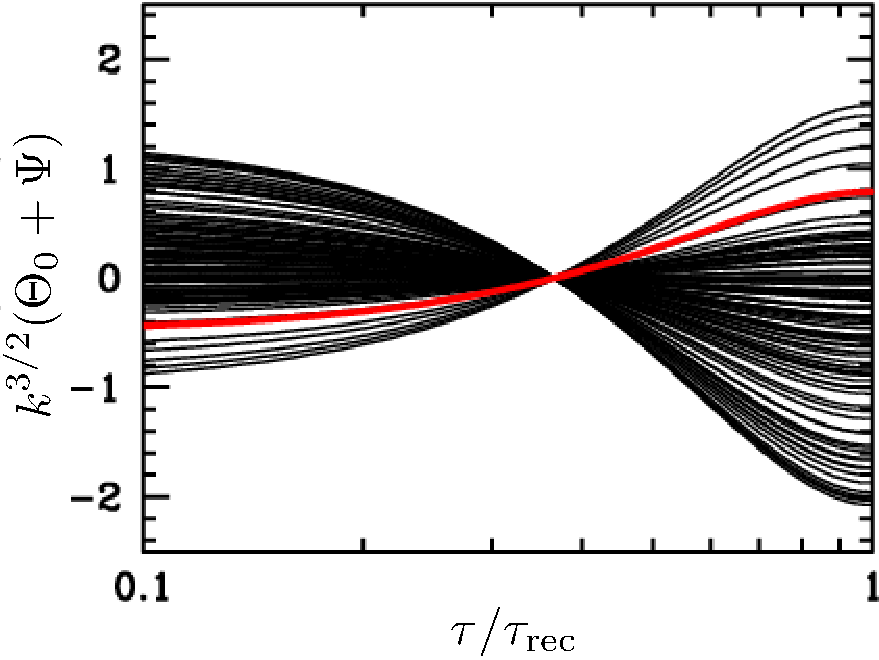
\includegraphics[width=.45\textwidth]{manymodes}
        \hspace{0.2cm}
                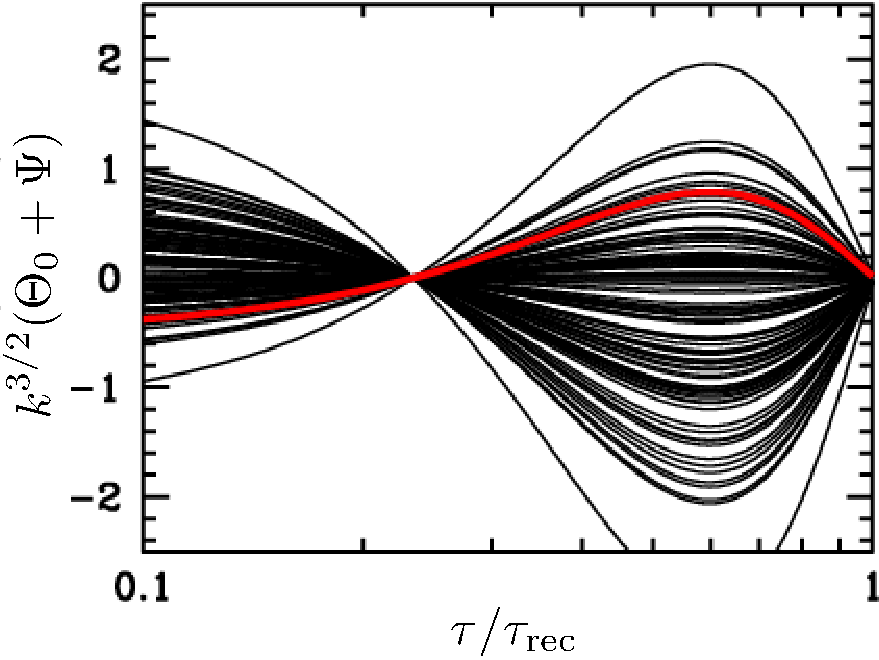
\includegraphics[width=.45\textwidth]{manytrough}
    \caption{\small 同じ波長をもつモードの時間発展．再結合は$\tau = \tau_{\rm rec}$で起こる．左図はCMB角度パワースペクトルの第1ピークに対応する波長を，右図は最初の谷に対応する波長を示す．すべてのモードは同じ位相から出発するため，左のモードはすべて再結合時に最大振幅となり，右のモードはすべて再結合時にゼロになる．これがCMBパワースペクトルのピークを説明する．}
    \label{fig:manymodes}
\end{figure}

\begin{figure}[h!]
    \centering
       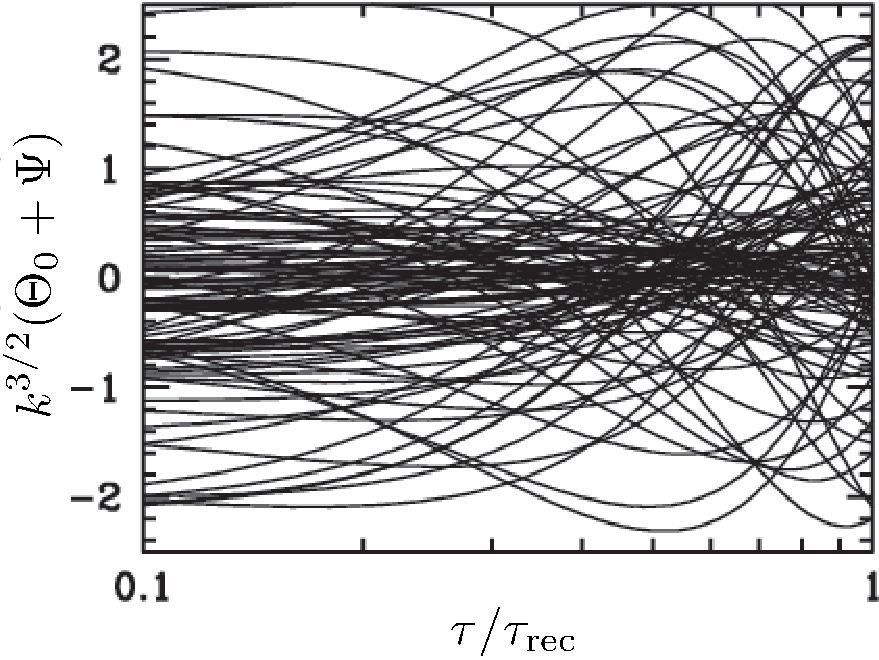
\includegraphics[width=.45\textwidth]{dec1}
         \hspace{0.2cm}
        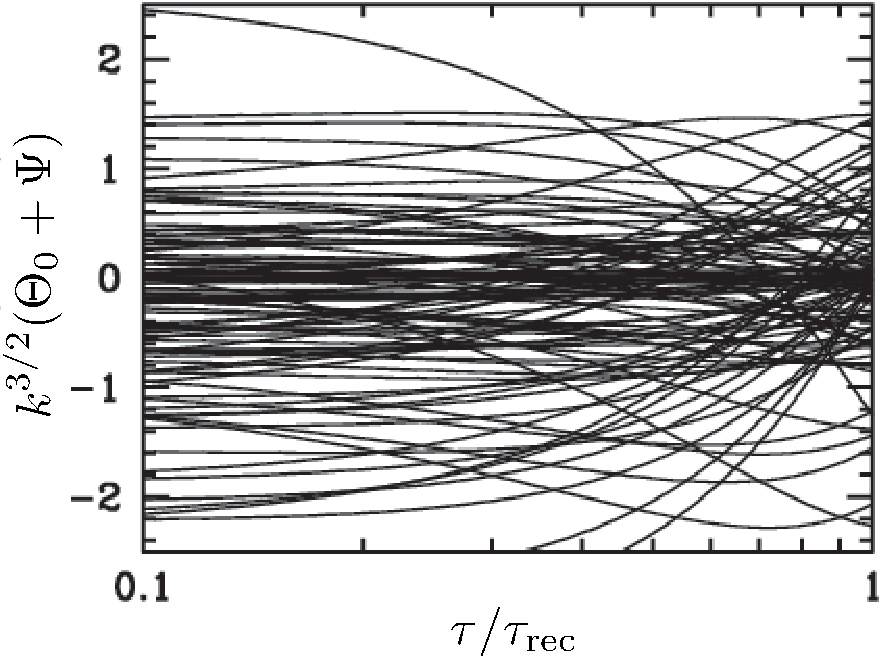
\includegraphics[width=.45\textwidth]{decoher}
    \caption{\small 図\ref{fig:manymodes}と同じ二つの波長に対応するモード．ただし，今度は初期位相がランダムである．CMBの角度方向のピーク構造が消えてしまうことがわかる．}
    \label{fig:decoher}
\end{figure}



\subsubsection{TEスペクトルの$\ell < 100$}

懐疑的な人は，上の議論だけでは納得しないかもしれない．CMB温度揺らぎスペクトルの山と谷は，角度スケール$\theta < 1^\circ$に対応する$\ell >200$にある．これらのスケールはすべて，再結合時には地平線の内側にあった．したがって，因果律に従いながらも「余弦モード」だけを生成する構造形成理論を組み立てることは，原理的には可能である（1990年代には実際に試みられた）．そのような理論は，インフレーションに頼らずにCMBのピークを説明する．最も美しい考え方とは言い難いが，論理的な可能性としては排除できない．

しかし，CMB偏光を考えると，このように高度に調整したインフレーションの代替理論さえも排除できることを，ここで示す．
図\ref{fig:TE}を見ると，CMB温度揺らぎと$E$モード偏光の相互相関は，$100 < \ell < 200$付近に負のピークをもつ．この反相関信号も位相のコヒーレンスの結果だが，今度のスケールは再結合時には地平線の内側に{\it なかった}．したがって，この信号を生成できる（$\tau =0$以降の）因果的な機構は{\it 存在しない}．共動地平線の縮小によって地平線からの退出と再突入が起こる，インフレーションのようなものを考えざるをえない．\footnote{ここで，共動ハッブル半径$1/(aH)$を縮小させる方法が二つあることを述べておく．インフレーション中は$H$がほぼ一定で，スケール因子$a$が指数関数的に成長する．しかし，{\it 収縮する}時空でも，$H$が時間とともに増大すれば地平線を縮小できる．これがエクピロティック／循環宇宙論\cite{Steinhardt:2002ih, Steinhardt:2001st, Buchbinder:2007ad}で用いられる機構である．共動ハッブルスケールの時間発展で見ると，インフレーションとエクピロティック模型は非常によく似ているが，重要な違いがある．例えば，エクピロティック模型では，収縮期を通常のビッグバン膨張に接続することが課題となる．}

Dodelsonは次のように説明している\cite{Dodelson:2003ip}．
\begin{quote}
再結合時には，［密度場の単極子（$T$の源）と双極子（$E$の源）の位相差によって］，両者の積は$100< \ell < 200$で負となり，より小さなスケールでは$\ell \sim 400$まで正となる．しかし，これはまさにWMAPが観測したものである！ 単極子と双極子が再結合時に互いに位相をずらしていたことの明確な証拠がある．

この証拠は，小スケールのモード（$\ell > 200$）についても刺激的である．音響ピークが位相のコヒーレンスを示すのと同様に，偏光と温度の相互相関は，双極子のコヒーレンスも物語っている．これは再結合時のプラズマについてのわれわれの描像を確かなものにする．
しかし，より大きなスケールのモード（$\ell < 200$）からの証拠は，まさに驚異的である．これらのモードは，再結合時には地平線の内側になかったからである．したがって，位相が揃いうる{\it 唯一}の方法は，因果的に接触していた時代に，何らかの原始的な機構がその仕事をしたというものである．インフレーションは，まさにそのような機構である．
\end{quote}

%TE spectrum proves that fluctuations are superhorizon at recombination.

\subsectionlink{スケール不変性，ガウス性，断熱性}
\label{sec:obs:source-duplicate-1}

次に，原始揺らぎに対する定量的な制限を説明する．
最も単純なインフレーション模型は，スカラー摂動がほぼ{\it スケール不変}，{\it ガウス的}，{\it 断熱的}であると予言する．本節では，理論のこれらの基本的な予言に対する最新の定量的制限を示す．

%Inflation predicts correlations of scalar modes $\R$ and tensor modes $h$.If the perturbations are gaussian, the correlations are completely determined by the power spectra $P_\R(k)$ and $P_h(k)$.

\vspace{0.5cm}
\begin{table}[h!]
\begin{center}
\begin{tabular}{||c|c|c||}
\hline \hline
{\small \bf パラメータ} & {\small {\sl WMAP} 5年観測} & {\small {\sl WMAP}+BAO+SN} \\
\hline
{\small $n_s$} & {\small $0.963_{-0.015}^{+0.014}$} & {\small $0.960_{-0.013}^{+0.013}$} \\
\hline
{\small $n_s$} & {\small $0.986 \pm 0.022$} & {\small $0.970 \pm 0.015$} \\
 {\small $r$} & {\small $<0.43$} & {\small $<0.22$} \\
\hline
 {\small $n_s$} & {\small $1.031_{-0.055}^{+0.054}$} & {\small $1.017_{-0.043}^{+0.042}$} \\
{\small  $\alpha_s$} & {\small $-0.037 \pm 0.028$} & {\small $-0.028_{-0.020}^{+0.020}$} \\
\hline
{\small $n_s$} & {\small $1.087_{-0.073}^{+0.072}$} & {\small $1.089_{-0.068}^{+0.070}$} \\
 {\small $r$} & {\small $<0.58$} & {\small $<0.55$} \\
{\small $\alpha_s$} & {\small $-0.050 \pm 0.034$} & {\small $-0.058 \pm 0.028$} \\
\hline \hline
\end{tabular}
\caption{ \label{tab:param} べき乗則によるパラメータ化における，原始パワースペクトルに対する{\sl WMAP} 5年観測の制限\cite{WMAP5}．平坦な$\Lambda$CDM模型の他のすべてのパラメータについて周辺化した，($n_s$)，($n_s$, $r$)，$(n_s, \alpha_s)$，($n_s$, $r$, $\alpha$)の結果を示す．}
\end{center}
\end{table}


\subsubsection{スペクトル指数}

上で詳しく説明したように，CMBの観測は，インフレーションが生成する曲率摂動$\R$のスペクトルに関係する．
\beq
\fbox{$\displaystyle
C_\ell^{TT}, C_\ell^{TE}, C_\ell^{EE} \quad \Rightarrow \quad P_\R(k) $}\, .
\eeq
ここでは，標準的なべき乗則のパラメータ化における，$P_\R(k)$に対する最新の定量的制限を示す．
\beq
\Delta^2_{\rm s}(k) \equiv \frac{k^3}{2\pi^2} P_\R(k) = A_{\rm s} \left(\frac{k}{k_\star} \right)^{n_{\rm s}-1} \, .
\eeq
$n_{\rm s}$の測定はテンソル・スカラー比$r$と縮退しているので，$n_{\rm s}$への制限は$n_{\rm s}$-$r$平面上の信頼領域として示されることが多い．
スカラー・スペクトル指数に対する最新のWMAP 5年観測の制限を，図\ref{fig:WMAP5}と表\ref{tab:param}に示す．
二つの事実に注目できる．
i) スペクトルは，インフレーションが予言するように，ほぼスケール不変$n_{\rm s} \approx 1$である．
ii) スペクトルが完全にはスケール不変ではなく，わずかに赤い$n_{\rm s} < 1$ことを示唆する興味深い兆候が，すでにある．このスケール不変性からのずれは，インフレーション膨張の詳細な時間依存性に対する最初の検証を与える．実際，{\bf 第2講}で見たように，インフレーションはこのパーセント程度のスケール不変性からのずれを予言する．\footnote{インフレーションが終わるには，ハッブルパラメータ$H$が時間とともに変化しなければならない．この時間依存性は，各揺らぎのモードが地平線を退出するときの条件を変え，そのため揺らぎのスケール依存性へと変換される．}
\begin{figure}[h!]
    \centering
        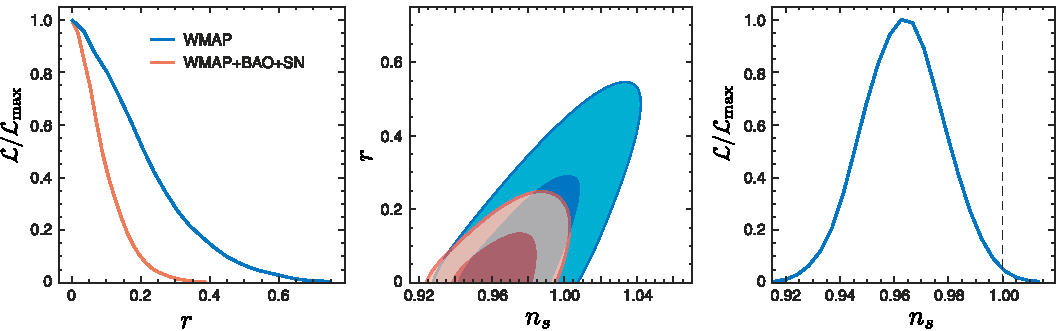
\includegraphics[width=.95\textwidth]{WMAP5_ns_r}
   \caption{インフレーションのパラメータ$n_s$と$r$に対する{\sl WMAP} 5年観測の制限\cite{WMAP5}．{\sl WMAP}だけの結果は青で，{\sl WMAP}に他の宇宙論的観測を加えた制限は赤で示す．
第3の図では，$r$は無視できると仮定している．
}%\newline [{\tt Placeholder.} {\tt Figure will be updated.}]}
    \label{fig:WMAP5}
\end{figure}



\subsubsection{ガウス性}

$\R$がガウス的なら，パワースペクトル$P_\R(k)$（実空間での2点相関）で話は完結する．
しかし，$\R$が{\it 非ガウス的}なら，揺らぎはゼロでないバイスペクトル$B_\R(k_1, k_2, k_3)$（実空間での3点相関に対応）をもつ．
ガウス的である仕方は一つしかないが，非ガウス的である仕方は多くあるので，非ガウス性への制限を述べるのは少し難しい．
非ガウス性の最も簡単な形の一つは，次のパラメータ化で記述される．
\beq
\label{equ:local2}
\R({\bf x}) = \R_g({\bf x}) + \frac{3}{5} f_{\rm NL} \star \R_g^2({\bf x})\, .
\eeq
ここで，$\R_g$はガウス的である．この非ガウス性の{\it 局所型模型}では，情報は一つの数$f_{\rm NL}$にまとめられる．
Smith，Senatore，Zaldarriaga\cite{Smith:2009jr}による$f_{\rm NL}$の最新の制限は，
\beq
\label{equ:smith}
- 4 \ < \ f_{\rm NL} \ < \ 80 \quad \text{（信頼水準} \ \ 95\% \ \text{）}\, .
\eeq
$f_{\rm NL}$が100程度の値であることは，式(\ref{equ:local2})の$\R_g \sim 10^{-5}$への0.1\%の補正に対応することに注意しよう．
したがって，制限(\ref{equ:smith})は，CMBが0.1\%の精度でガウス的であることを意味する！ これは，通常インフレーションの勝利として称賛される，宇宙の曲率への制限よりも厳しい．
CMBはきわめてガウス的だが，必ずそうでなければならなかったわけではない．
しかし，インフレーションが正しければ，観測されるガウス性はむしろ自然な帰結である．\footnote{非ガウス性は，インフラトン場の{\it 相互作用}の尺度である．しかし，スローロールの力学が成り立つには，インフラトンの自己相互作用が非常に弱くなければならず（ポテンシャルが非常に平坦），非ガウス性は必然的に小さく，$f_{\rm NL} \sim {\cal O}(0.01)$となる\cite{malda}．}

\subsubsection{断熱性}

単一場インフレーションでは，大きなスケール（空間勾配を無視できるスケール）でのインフラトン場の揺らぎは，一様な背景場の軌道に沿った局所的な前進または後退と同一視できる．インフラトンの軌道に沿ったこのずれは，インフレーション後の宇宙の各領域の全密度に影響するが，異なる成分の相対密度の変動を生むことはできない．
したがって，単一場インフレーションは，全体の曲率摂動$\R$で特徴付けられる，純粋に{\it 断熱的}な原始密度摂動を生成する．
これは，宇宙流体（光子，ニュートリノ，バリオン，冷たい暗黒物質（CDM）粒子）のすべての摂動が，同じ曲率摂動$\R$から生じ，断熱性の性質$\delta(n_m/n_r) =0$，または次式を満たすことを意味する．
\beq
\label{equ:ad}
\frac{\delta \rho_m}{\rho_m} = \frac{3}{4} \frac{\delta \rho_r}{\rho_r}\, ,
\eeq
ここで，添字$m$は非相対論的な成分（バリオンまたはCDM）をまとめて表し，$r$は相対論的な成分（光子またはニュートリノ）を表す．
最新のデータには，条件(\ref{equ:ad})の破れは見られない\cite{WMAP5}．
そのような破れが見つかれば，多場インフレーションの明確な徴候となる（\S\ref{sec:iso}参照）．

\subsectionlink{スローロール模型の検証}

図\ref{fig:nsr}に，最も単純な単一場スローロール・インフレーション模型のいくつかに対する，現在の観測的制限を示す（{\bf 第1講}参照）．
将来の測定は，許される模型のパラメータ空間を大幅に狭めるだろう．

\begin{figure}[h!]
    \centering
        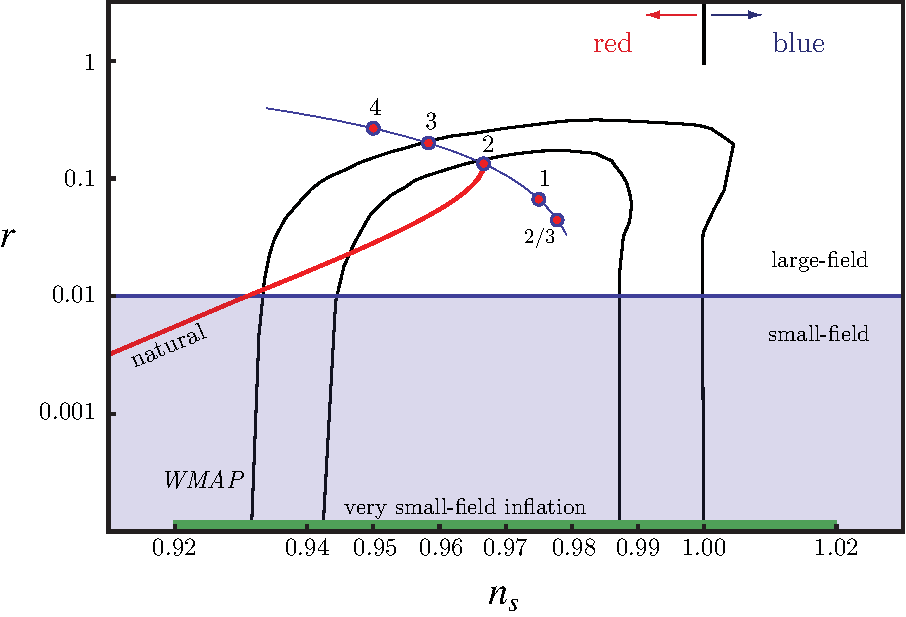
\includegraphics[width=.65\textwidth]{nsr}
   \caption{$n_s$-$r$平面上の単一場スローロール模型への制限．$r$の値は，模型における場の変位が大きいか小さいかを決める．$n_s$の値は，スカラー・スペクトルを赤いものと青いものに分類する．$r$と$n_s$の値の組合せにより，観測可能な宇宙が地平線を退出したとき，ポテンシャルの曲率が正（$\eta_{\rm v} > 0$）だったか負（$\eta_{\rm v} < 0$）だったかが決まる．
また，$n_s$と$r$に対する{\sl WMAP} 5年観測の制限\cite{WMAP5}と，単一場スローロール・インフレーションの代表的ないくつかの模型の予言も示す．
%\newline
{\it カオス的インフレーション}：$\lambda_p\, \phi^p$．一般の$p$（細い実線）と$p=4, 3, 2, 1, \frac{2}{3}$（{\large $\bullet$}）を示す．$p=2$~\cite{Nflation}，$p=1$~\cite{MSW}，$p=\frac{2}{3}$~\cite{Silverstein:2008sg}の模型は，最近，弦理論から得られた．
%\newline
{\it 自然インフレーション}：$V_0 [1-\cos(\phi/\mu)]$（実線）．
%{\it hill-top inflation}: $V_0 [1-(\phi/\mu)^2] + \dots$ (solid line);
%\newline
{\it 非常に小さな場のインフレーション}：非常に小さなテンソル振幅$r \ll 10^{-4}$をもつインフレーション模型（緑の帯）．弦理論における例として，ワープしたDブレーン・インフレーション\cite{KKLMMT, Baumann:2007ah, Baumann:2008kq}，ケーラー・インフレーション\cite{Conlon:2005jm}，レーストラック・インフレーション\cite{BlancoPillado:2006he}がある．}
    \label{fig:nsr}
\end{figure}


\sectionlink{インフレーションの将来の検証}

インフレーションの枠組みを本格的に検証する作業は，まだ始まったばかりである．
宇宙の平坦性と，密度揺らぎのほぼスケール不変な性質，ガウス性，断熱性は，インフレーションを支持する心強い証拠である\footnote{どの段階でも，インフレーションという考え方全体を反証する測定が得られた可能性があることに注意しよう．}が，インフレーションが実際に起こったことの証明ではない．\footnote{カール・ポパーは理論を決して証明できないと教えたのに，「証明」という言葉を使ってしまったことは承知している．}
そこで未来に目を向け，将来の実験がインフレーションの物理をどのようにさらに検証できるかを説明しよう．


\subsectionlink{テンソルモードの振幅}

おそらく，インフレーションの証拠として単独で最も重要なのは，原始テンソル振幅の測定であろう．
上で示したように，原始CMBの$B$モードが検出されれば，それをインフレーションの重力波以外で説明することは事実上不可能である\cite{BauZal}．
\beq
\fbox{$\displaystyle
C_\ell^{BB} \quad \Rightarrow \quad P_h(k) $}\, ,
\eeq
ここで，
\beq
\Delta^2_{\rm t}(k) \equiv \frac{k^3}{2\pi^2} P_h(k) = A_{\rm t} \left(\frac{k}{k_\star} \right)^{n_{\rm t}} \, .
\eeq
また，{\bf 第2講}では，テンソル振幅$A_t$がインフレーションのエネルギースケールに直接結び付くことを説明した．
インフレーションの物理に関する単独の手掛かりとして，これ以上に重要で，インフレーションの理論家が強く望むものがあるだろうか．
さらに，テンソルモードの検出は，インフラトン場が場の空間でプランクスケールを超える距離を動いたことを意味し，弦理論家や量子重力の愛好家に，インフラトン・ポテンシャルへのプランクスケールで抑制された補正を真剣に考えさせるだろう（{\bf 第5講}参照）．

\subsectionlink{スカラーモードのスケール依存性}

スペクトル指数$n_{\rm s}$のスケールによる変化（スペクトル指数の「ランニング」とも呼ばれる）は，スローロールの2次で初めて生じるので，小さいと期待される．
\beq
\alpha_{\rm s} \equiv \frac{d n_{\rm s}}{d \ln k} \sim {\cal O}(\varepsilon^2)\, .
\eeq
一方，予想に反する大きな正または負のランニングが見つかれば，インフレーションと摂動生成に関する最も単純な考え方の一部を見直す必要がある．

\subsectionlink{テンソルモードのスケール依存性}

インフレーションに由来する原始テンソル揺らぎの振幅を測定することは，観測上の大きな挑戦となる．
テンソル振幅が現在の上限に近くない限り，そのスケール依存性まで測定することを期待するのは現実的でないように思われる．
単一場スローロール模型では，テンソル・スカラー比$r$とテンソル・スペクトル指数$n_{\rm t}$は，{\it 整合性関係}によって結び付けられる．
\beq
\label{equ:cons}
r = - 8 n_{\rm t}\, .
\eeq
式(\ref{equ:cons})を測定することは，単一場スローロール・インフレーションを反証するための別の方法となる．

\subsectionlink{非ガウス性}

原始揺らぎは，非常に高い精度でガウス的である．
しかし，これから説明するように，わずかな非ガウス性にも，インフレーションの作用について膨大な情報が含まれる．
インフレーションの揺らぎの3点関数が，非ガウス統計を診断する主要な手段であることはすでに述べた．
運動量空間では，3点相関関数は一般に次のように書ける．
\beq
\langle \R_{{\bf k}_1} \R_{{\bf k}_2} \R_{{\bf k}_3} \rangle = (2\pi)^3\, \delta({\bf k}_1 + {\bf k}_2 + {\bf k}_3) \ f_{\rm NL} \ F(k_1, k_2, k_3)\, .
\eeq
ここで，$f_{\rm NL}$は非ガウス性の振幅を定義する無次元パラメータであり，関数$F(k_1, k_2, k_3)$が運動量依存性を担う．$f_{\rm NL}$の振幅と符号，および$F(k_1,k_2,k_3)$の形とスケール依存性は，非ガウス性を生成する相互作用の詳細に依存する．このため，3点関数は初期宇宙の模型を調べ，区別するための強力な道具となる\cite{NGreview}．

二つの非常に異なる機構によって，二つの単純で異なる形$F(k_1, k_2, k_3)$が生成される\cite{Babich_etal_04}．{\em 局所型の形}は多場模型に特徴的であり，その名は原始曲率摂動$\R$の実空間での表式に由来する．
\begin{equation}
\label{local} \R({\bf x}) = \R_g({\bf x}) + \frac{3}{5} f_{\rm NL}^{\rm local} \R_g({\bf x})^2\, ,
\end{equation}
ここで，$\R_g({\bf x})$はガウス確率場である．この表式をフーリエ変換すると，信号は$k_3 \ll k_1,k_2$という「押しつぶされた」三角形に集中することがわかる．局所型非ガウス性は，等曲率場（後述）の揺らぎが曲率摂動へ変換される多場模型で生じる．この変換は地平線の外側で起こり，そこでは勾配が重要でないため，式(\ref{local})の形の非線形性が生成される．この種類の具体的な模型には，多場インフレーション\cite{BMRmulti, Bernardeau:2002jy, Bernardeau:2002jf, Sasaki:2008uc, Naruko:2008sq, Byrnes:2008wi, Byrnes:2006fr, Langlois:2008vk, Valiviita:2008zb, Assadullahi:2007uw, Valiviita:2006mz, Vernizzi:2006ve, Allen:2005ye}，カーバトン・シナリオ\cite{Linde:1996gt, Lyth_etal03}，非一様再加熱\cite{Dvali:2003em, Kofman:2003nx}，新エクピロティック模型\cite{Creminelli:2007aq,Koyama_etal07,Buchbinder_etal07, Lehners:2007wc,Lehners:2008my, Koyama:2007ag, Koyama:2007mg}がある．
%In these cases, $|f_{\rm NL}^{\rm local}|$ is model-dependent but generically larger than $5-10$.

第2の重要な形は，$k_1 \sim k_2 \sim k_3$の配置で最大になるため，{\em 正三角形型}と呼ばれる．正三角形型は，DBIインフレーション\cite{Alishahiha:2004eh}，ゴースト・インフレーション\cite{GhostInflation,Senatore:2004rj}，およびより一般的な音速の小さい模型\cite{Creminelli:2003iq, Chen:2006nt}など，非正準運動項をもつ単一場模型によって生成される．

\subsectionlink{等曲率揺らぎ}
\label{sec:iso}

複数の場をもつインフレーション模型では，摂動は必ずしも断熱的ではない．
場が複数あると，全密度，したがって空間曲率に摂動がなくても，背景の軌道に直交する揺らぎが，異なる物質成分の相対密度に影響を与えうる\cite{Gordon:2000hv}．
このような{\it 等曲率}摂動（非断熱摂動またはエントロピー摂動とも呼ばれる）には，さまざまな可能性がある．例えば，CDMと光子の間の相対的な摂動を定義できる．
\beq
{\cal S}_m \equiv \frac{\delta \rho_m}{\rho_m} - \frac{3}{4} \frac{\delta \rho_\gamma}{\rho_\gamma}\, .
\eeq
断熱摂動と等曲率摂動は，CMB揺らぎに異なるピーク構造を生む．
したがって，CMB測定によって揺らぎの種類を区別でき，実際，等曲率摂動が（存在するとしても）劣勢の成分でなければならないことが，すでに示されている．

等曲率摂動は断熱摂動と相関している可能性がある．これを表すため，次の相関パラメータを定義する．
\beq
\beta \equiv \frac{P_{{\cal S} {\cal R}}}{\sqrt{P_{\cal S} P_\R}}\, ,
\eeq
ここで，$P_{\cal R}$と$P_{\cal S}$は，それぞれ断熱揺らぎと等曲率揺らぎのパワースペクトルであり，$P_{{\cal S} \R}$はその相互相関である．
2種類の摂動の相対振幅を係数$\alpha$でパラメータ化する．
\beq
\frac{P_{\cal S}}{P_\R} \equiv \frac{\alpha}{1-\alpha}\, ,
\eeq
等曲率成分の寄与への現在の制限は，無相関の場合（$\beta =0$）には$\alpha_0 < 0.067$（信頼水準96\%），完全に反相関の場合（$\beta = -1$）には$\alpha_{-1} < 0.0037$（信頼水準95\%）である．

等曲率摂動の振幅の理論予言は，模型に強く依存するため複雑になる．等曲率振幅は，多場インフレーションの力学だけでなく，インフレーション後の時間発展にも依存する．インフレーション後にすべての粒子種が熱平衡にあり，それらの局所密度が（化学ポテンシャルがゼロで）温度だけによって一意に決まるなら，原始摂動は断熱的となる\cite{Lyth:2002my,Weinberg04b}．したがって，原始等曲率モードが存在するためには，少なくとも一つの場が，存在量が熱平衡によって決まらない粒子種（例えば脱結合後のCDM），またはバリオン数やレプトン数のような保存量子数に従う粒子種へ崩壊しなければならないことに注意するのが重要である．

\newpage
\sectionlink{{\sl まとめ}：第3講}

\vskip 10pt
宇宙マイクロ波背景放射（CMB）と大規模構造（LSS）の観測は，構造の種となる原始揺らぎのスペクトルを制限するために用いられる．
これにより，CMBとLSSの実験は初期宇宙を探る手段となる．
インフレーション期についてのこの情報を取り出すには，揺らぎの後期の時間発展を考慮しなければならない．
これは，{\sf CMBFAST}や{\sf CAMB}などの数値計算コードで行う．

\vskip 6pt
現在の観測は，インフレーションの基本的な予言と見事に一致している．
宇宙は平坦であり，ほぼスケール不変でガウス的かつ断熱的な密度揺らぎのスペクトルをもつ．揺らぎは，再結合時に地平線より大きかったスケールで，ゼロでない相関を示す．さらに，CMBスペクトルのピーク構造は，揺らぎがコヒーレントな位相で生成されたことの証拠である．

\vskip 6pt
インフレーションの将来の検証は，主としてCMB偏光の測定から得られるだろう．
CMB偏光の$B$モードは，インフレーションの重力波に特有の徴候である．
$B$モードの振幅は，インフレーションのエネルギースケールを直接測る．
さらに，非ガウス性の測定は，インフラトン場の相互作用を制限することにより，インフレーションの物理について豊富な情報をもたらす可能性がある．

\vskip 6pt
最後に，次の測定結果は，単一場スローロール・インフレーションを反証する．
\begin{itemize}
\item 大きな非ガウス性，$f_{\rm NL} > 1$．
\item ゼロでない等曲率摂動，$\alpha \ne 0$．
\item スカラー・スペクトルの大きなランニング，$|\alpha_{\rm s}| > 0.001$．
\item テンソルの整合性関係の破れ，$r \ne - 8 n_{\rm t}$．
\end{itemize}



%\newpage
%\sectionlink{{\sl Problem Set}: Lecture 3}

%\vskip 10pt


\newpage
%\part{Lecture 4: Advanced Topic: Non-Gaussianity}
